\documentclass[]{article}
\usepackage{lmodern}
\usepackage{amssymb,amsmath}
\usepackage{ifxetex,ifluatex}
\usepackage{fixltx2e} % provides \textsubscript
\ifnum 0\ifxetex 1\fi\ifluatex 1\fi=0 % if pdftex
  \usepackage[T1]{fontenc}
  \usepackage[utf8]{inputenc}
\else % if luatex or xelatex
  \ifxetex
    \usepackage{mathspec}
  \else
    \usepackage{fontspec}
  \fi
  \defaultfontfeatures{Ligatures=TeX,Scale=MatchLowercase}
\fi
% use upquote if available, for straight quotes in verbatim environments
\IfFileExists{upquote.sty}{\usepackage{upquote}}{}
% use microtype if available
\IfFileExists{microtype.sty}{%
\usepackage{microtype}
\UseMicrotypeSet[protrusion]{basicmath} % disable protrusion for tt fonts
}{}
\usepackage[margin=1in]{geometry}
\usepackage{hyperref}
\hypersetup{unicode=true,
            pdftitle={Laborator 1},
            pdfborder={0 0 0},
            breaklinks=true}
\urlstyle{same}  % don't use monospace font for urls
\usepackage{color}
\usepackage{fancyvrb}
\newcommand{\VerbBar}{|}
\newcommand{\VERB}{\Verb[commandchars=\\\{\}]}
\DefineVerbatimEnvironment{Highlighting}{Verbatim}{commandchars=\\\{\}}
% Add ',fontsize=\small' for more characters per line
\usepackage{framed}
\definecolor{shadecolor}{RGB}{248,248,248}
\newenvironment{Shaded}{\begin{snugshade}}{\end{snugshade}}
\newcommand{\KeywordTok}[1]{\textcolor[rgb]{0.13,0.29,0.53}{\textbf{#1}}}
\newcommand{\DataTypeTok}[1]{\textcolor[rgb]{0.13,0.29,0.53}{#1}}
\newcommand{\DecValTok}[1]{\textcolor[rgb]{0.00,0.00,0.81}{#1}}
\newcommand{\BaseNTok}[1]{\textcolor[rgb]{0.00,0.00,0.81}{#1}}
\newcommand{\FloatTok}[1]{\textcolor[rgb]{0.00,0.00,0.81}{#1}}
\newcommand{\ConstantTok}[1]{\textcolor[rgb]{0.00,0.00,0.00}{#1}}
\newcommand{\CharTok}[1]{\textcolor[rgb]{0.31,0.60,0.02}{#1}}
\newcommand{\SpecialCharTok}[1]{\textcolor[rgb]{0.00,0.00,0.00}{#1}}
\newcommand{\StringTok}[1]{\textcolor[rgb]{0.31,0.60,0.02}{#1}}
\newcommand{\VerbatimStringTok}[1]{\textcolor[rgb]{0.31,0.60,0.02}{#1}}
\newcommand{\SpecialStringTok}[1]{\textcolor[rgb]{0.31,0.60,0.02}{#1}}
\newcommand{\ImportTok}[1]{#1}
\newcommand{\CommentTok}[1]{\textcolor[rgb]{0.56,0.35,0.01}{\textit{#1}}}
\newcommand{\DocumentationTok}[1]{\textcolor[rgb]{0.56,0.35,0.01}{\textbf{\textit{#1}}}}
\newcommand{\AnnotationTok}[1]{\textcolor[rgb]{0.56,0.35,0.01}{\textbf{\textit{#1}}}}
\newcommand{\CommentVarTok}[1]{\textcolor[rgb]{0.56,0.35,0.01}{\textbf{\textit{#1}}}}
\newcommand{\OtherTok}[1]{\textcolor[rgb]{0.56,0.35,0.01}{#1}}
\newcommand{\FunctionTok}[1]{\textcolor[rgb]{0.00,0.00,0.00}{#1}}
\newcommand{\VariableTok}[1]{\textcolor[rgb]{0.00,0.00,0.00}{#1}}
\newcommand{\ControlFlowTok}[1]{\textcolor[rgb]{0.13,0.29,0.53}{\textbf{#1}}}
\newcommand{\OperatorTok}[1]{\textcolor[rgb]{0.81,0.36,0.00}{\textbf{#1}}}
\newcommand{\BuiltInTok}[1]{#1}
\newcommand{\ExtensionTok}[1]{#1}
\newcommand{\PreprocessorTok}[1]{\textcolor[rgb]{0.56,0.35,0.01}{\textit{#1}}}
\newcommand{\AttributeTok}[1]{\textcolor[rgb]{0.77,0.63,0.00}{#1}}
\newcommand{\RegionMarkerTok}[1]{#1}
\newcommand{\InformationTok}[1]{\textcolor[rgb]{0.56,0.35,0.01}{\textbf{\textit{#1}}}}
\newcommand{\WarningTok}[1]{\textcolor[rgb]{0.56,0.35,0.01}{\textbf{\textit{#1}}}}
\newcommand{\AlertTok}[1]{\textcolor[rgb]{0.94,0.16,0.16}{#1}}
\newcommand{\ErrorTok}[1]{\textcolor[rgb]{0.64,0.00,0.00}{\textbf{#1}}}
\newcommand{\NormalTok}[1]{#1}
\usepackage{longtable,booktabs}
\usepackage{graphicx,grffile}
\makeatletter
\def\maxwidth{\ifdim\Gin@nat@width>\linewidth\linewidth\else\Gin@nat@width\fi}
\def\maxheight{\ifdim\Gin@nat@height>\textheight\textheight\else\Gin@nat@height\fi}
\makeatother
% Scale images if necessary, so that they will not overflow the page
% margins by default, and it is still possible to overwrite the defaults
% using explicit options in \includegraphics[width, height, ...]{}
\setkeys{Gin}{width=\maxwidth,height=\maxheight,keepaspectratio}
\IfFileExists{parskip.sty}{%
\usepackage{parskip}
}{% else
\setlength{\parindent}{0pt}
\setlength{\parskip}{6pt plus 2pt minus 1pt}
}
\setlength{\emergencystretch}{3em}  % prevent overfull lines
\providecommand{\tightlist}{%
  \setlength{\itemsep}{0pt}\setlength{\parskip}{0pt}}
\setcounter{secnumdepth}{5}
% Redefines (sub)paragraphs to behave more like sections
\ifx\paragraph\undefined\else
\let\oldparagraph\paragraph
\renewcommand{\paragraph}[1]{\oldparagraph{#1}\mbox{}}
\fi
\ifx\subparagraph\undefined\else
\let\oldsubparagraph\subparagraph
\renewcommand{\subparagraph}[1]{\oldsubparagraph{#1}\mbox{}}
\fi

%%% Use protect on footnotes to avoid problems with footnotes in titles
\let\rmarkdownfootnote\footnote%
\def\footnote{\protect\rmarkdownfootnote}

%%% Change title format to be more compact
\usepackage{titling}

% Create subtitle command for use in maketitle
\newcommand{\subtitle}[1]{
  \posttitle{
    \begin{center}\large#1\end{center}
    }
}

\setlength{\droptitle}{-2em}
  \title{Laborator 1}
  \pretitle{\vspace{\droptitle}\centering\huge}
  \posttitle{\par}
\subtitle{Introducere în R}
  \author{}
  \preauthor{}\postauthor{}
  \date{}
  \predate{}\postdate{}

\usepackage{booktabs}
\usepackage{longtable}
\usepackage{framed,color}
\definecolor{shadecolor}{RGB}{248,248,248}

\ifxetex
  \usepackage{letltxmacro}
  \setlength{\XeTeXLinkMargin}{1pt}
  \LetLtxMacro\SavedIncludeGraphics\includegraphics
  \def\includegraphics#1#{% #1 catches optional stuff (star/opt. arg.)
    \IncludeGraphicsAux{#1}%
  }%
  \newcommand*{\IncludeGraphicsAux}[2]{%
    \XeTeXLinkBox{%
      \SavedIncludeGraphics#1{#2}%
    }%
  }%
\fi

\newenvironment{rmdblock}[1]
  {\begin{shaded*}
  \begin{itemize}
  \renewcommand{\labelitemi}{
    \raisebox{-.7\height}[0pt][0pt]{
      {\setkeys{Gin}{width=2em,keepaspectratio}\includegraphics{images/icons/#1}}
    }
  }
  \item
  }
  {
  \end{itemize}
  \end{shaded*}
  }
\newenvironment{rmdcaution}
  {\begin{rmdblock}{caution}}
  {\end{rmdblock}}
\newenvironment{rmdinsight}
  {\begin{rmdblock}{insight}}
  {\end{rmdblock}}
\newenvironment{rmdexercise}
  {\begin{rmdblock}{exercise}}
  {\end{rmdblock}}
\newenvironment{rmdtip}
  {\begin{rmdblock}{tip}}
  {\end{rmdblock}}
  
%%%%%%%%%%%%%%%%%%%%%%%%%%%%%%%%%%%%%%%%%%%%%%%%%%%%%%%%%%%%%%%%%%%%%%%%%%%%%%%%%%%%%%%%%%%%%%%%%%%%%%%%%%%%%%%%%%%%%
\usepackage{subfigure}
\usepackage{booktabs}
\usepackage{slashbox}
\usepackage{color}
%%%%%%%%%%%%%%%%%%%%%%%%%%%%%%%%%%%%%%%%%%%%%%%%%%%%%%%%%%%%%%%%%%%%%%%%%%%%%%%%%%%%%%%%%%%%%%%%%%%%%%%%%%%%%%%%%%%%%
%CITEVA DEFINITII
\def\om{\omega}
\def\Om{\Omega}
\def\et{\eta}
\def\td{\tilde{\delta}}
\def\m{{\mu}}
\def\n{{\nu}}
\def\k{{\kappa}}
\def\l{{\lambda}}
\def\L{{\Lambda}}
\def\g{{\gamma}}
\def\a{{\alpha}}
\def\e{{\varepsilon}}
\def\b{{\beta}}
\def\G{{\Gamma}}
\def\d{{\delta}}
\def\D{{\Delta}}
\def\t{{\theta}}
\def\s{{\sigma}}
\def\S{{\Sigma}}
\def\z{{\zeta}}
\def\qed{\hfill\Box}
\def\ds{\displaystyle}
\def\mc{\mathcal}
%%%%%%%%%%%%%%%%%%%%%%%%%%%%%%%%%%%%%%%%%%%%%%%%%%%%%%%%%%%%%%%%%%%%%%%%%%%%%%%%%%%%%%%%%%%%%%%%%%%%%%%%%%%%%%%%%%%%%%
\def\1{{\mathbf 1}}
\def\CC{{\mathbb C}}
\def\VV{{\mathbb V}}
\def\RR{{\mathbb R}}
\def\QQ{{\mathbb Q}}
\def\ZZ{{\mathbb Z}}
\def\PP{{\mathbb P}}
\def\EE{{\mathbb E}}
\def\NN{{\mathbb N}}
\def\FF{{\mathbb F}}
%\def\SS{{\mathbb S}}
\def\MA{{\mathcal A}}
\def\MO{{\mathcal O}}
\def\MF{{\mathcal F}}
\def\ME{{\mathcal E}}
\def\MR{{\mathcal R}}
\def\MB{{\mathcal B}}
\def\MM{{\mathcal M}}
\def\MN{{\mathcal N}}
\def\MU{{\mathcal U}}
\def\MP{{\mathcal P}}
\def\MS{{\mathcal S}}
\def\MBS{{\mathbf S}}
\def\MX{{\bm{ \mathscr X}}}

% independent sign
\newcommand\independent{\protect\mathpalette{\protect\independenT}{\perp}}
\def\independenT#1#2{\mathrel{\rlap{$#1#2$}\mkern2mu{#1#2}}}

%%%%%%%%%%%%%%%%%%%%%%%%%%%%%%%%%%%%%%%%%%%%%%%%%%%%%%%%%%%%%%%%%%%%%%%%%%%%%%%%%%%%%%%%%%%%%%%%%%%%%%%%%%%%%%%%%%%%%
%Header and Footer
\usepackage{fancyhdr}

\pagestyle{fancy}
\fancyhf{}
\rhead{Universitatea din Bucure\c sti\\ Facultatea de Matematic\u a \c si Informatic\u a}
\lhead{\textit{Curs}: Probabilit\u a\c ti \c si Statistic\u a\\ \textit{Instructor}: A. Am\u arioarei}
\rfoot{Pagina \thepage}
\lfoot{Grupele: 241, 242, 243, 244}
%%%%%%%%%%%%%%%%%%%%%%%%%%%%%%%%%%%%%%%

\begin{document}
\maketitle

Obiectivul acestui laborator este de a prezenta o scurtă introducere în
programul \href{https://cran.r-project.org/}{R} (cu ajutorul interfeței
grafice \href{https://www.rstudio.com/}{RStudio}). O descriere detaliată
a acestui program precum și versiunile disponibile pentru descărcat se
găsesc pe site-ul
\href{http://www.r-project.org}{\texttt{www.r-project.org}}.

\section{Introducere}\label{introducere}

Programul \texttt{R} este un program \textbf{gratuit} destinat, cu
precădere, analizei statistice și prezintă o serie de avantaje:

\begin{itemize}
\tightlist
\item
  rulează aproape pe toate platformele și sistemele de operare
\item
  permite folosirea metodelor statistice clasice cu ajutorul unor
  funcții predefinite
\item
  este adoptat ca limbaj de analiză statistică în majoritatea domeniilor
  aplicate
\item
  prezintă capabilități grafice deosebite
\item
  permite utilizarea tehnicilor statistice de ultimă oră prin
  intermediul pachetelor dezvoltate de comunitate (în prezent sunt mai
  mult de 10000 de pachete)
\item
  are o comunitate foarte activă și în continuă creștere
\end{itemize}

\begin{figure}

{\centering 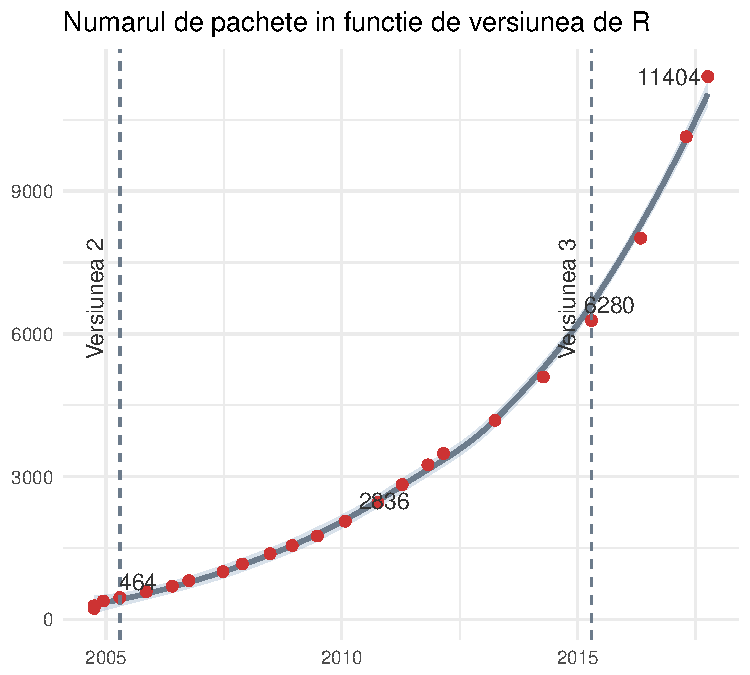
\includegraphics{Lab_1_pdf_files/figure-latex/unnamed-chunk-2-1} 

}

\caption{Numarul de pachete din R}\label{fig:unnamed-chunk-2}
\end{figure}

\subsection{\texorpdfstring{Interfața
\texttt{RStudio}}{Interfața RStudio}}\label{interfata-rstudio}

Interfața RStudio (vezi Figura 1) este compusă din patru ferestre:

\begin{itemize}
\tightlist
\item
  \emph{Fereastra de editare} (stânga sus): în această fereastră apar
  fișierele, de tip \texttt{script}, în care utilizatorul dezvoltă
  propriile funcții ori script-uri.\\
\item
  \emph{Fereastra de comandă} sau \emph{consola} (stânga jos): în
  această fereastră sunt executate comenzile R
\item
  \emph{Fereastra cu spațiul de lucru/istoricul} (dreapta sus): conține
  obiectele definite în memorie și istoricul comenzilor folosite
\item
  \emph{Fereastra de explorare} (dreapta jos): în această fereastră ne
  putem deplasa în interiorul repertoriului (tab-ul \emph{Files}), putem
  vedea graficele trasate (tab-ul \emph{Plots}) dar și pachetele
  instalate (tab-ul \emph{Packages}). De asemenea, tot în această
  fereastră putem să și căutăm documentația despre diferite funcții,
  folosind fereastra de ajutor (tab-ul \emph{Help}).
\end{itemize}

\begin{figure}

{\centering 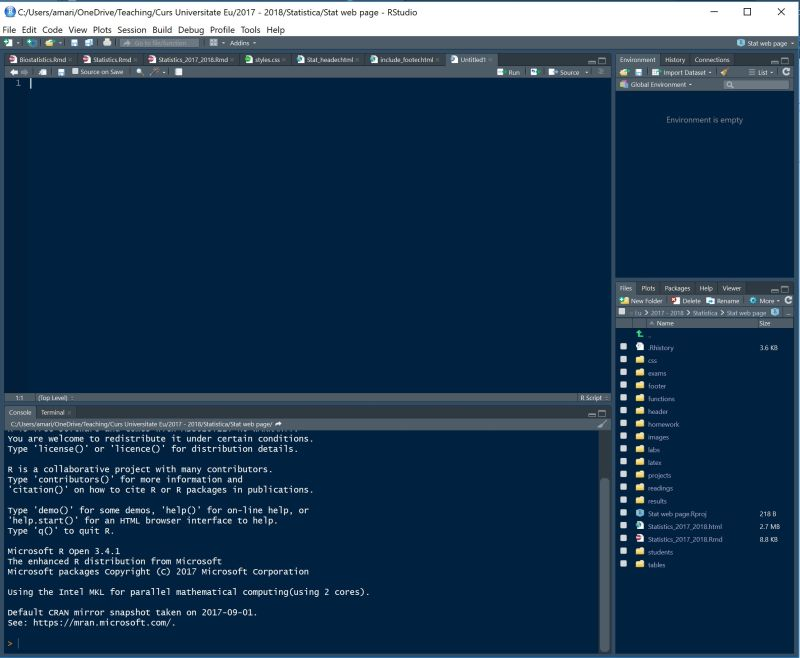
\includegraphics[width=11.11in]{images/lab1/RStudio2} 

}

\caption{Interfata RStudio}\label{fig:unnamed-chunk-3}
\end{figure}

\subsection{Pachetele ajutătoare}\label{pachetele-ajutatoare}

Pe lângă diferitele pachete conținute în versiunea de bază a programului
\texttt{R} se mai pot instala și pachete suplimentare. Pentru a instala
un pachet suplimentar se apelează comanda:

\begin{Shaded}
\begin{Highlighting}[]
\KeywordTok{install.packages}\NormalTok{(}\StringTok{"nume pachet"}\NormalTok{)}
\end{Highlighting}
\end{Shaded}

Odată ce pachetul este instalat, pentru a încărca pachetul, și prin
urmare funcțiile disponibile în acesta, se apelează comanda:

\begin{Shaded}
\begin{Highlighting}[]
\KeywordTok{library}\NormalTok{(}\StringTok{"nume pachet"}\NormalTok{)}
\end{Highlighting}
\end{Shaded}

Instalarea unui pachet se face o singură dată dar încărcarea acestuia
trebuie făcută de fiecare dată când lansăm o sesiune nouă.

\section{\texorpdfstring{Primele comenzi în
\texttt{R}}{Primele comenzi în R}}\label{primele-comenzi-in-r}

\subsection{Calcul elementar}\label{calcul-elementar}

Programul \texttt{R} poate fi folosit și pe post de calculator (mai
avansat). De exemplu putem face calcule elementare

\begin{Shaded}
\begin{Highlighting}[]
\DecValTok{5} \OperatorTok{-}\StringTok{ }\DecValTok{1} \OperatorTok{+}\StringTok{ }\DecValTok{10}
\end{Highlighting}
\end{Shaded}

\begin{verbatim}
## [1] 14
\end{verbatim}

\begin{Shaded}
\begin{Highlighting}[]
\DecValTok{7} \OperatorTok{*}\StringTok{ }\DecValTok{10} \OperatorTok{/}\StringTok{ }\DecValTok{2}
\end{Highlighting}
\end{Shaded}

\begin{verbatim}
## [1] 35
\end{verbatim}

\begin{Shaded}
\begin{Highlighting}[]
\KeywordTok{exp}\NormalTok{(}\OperatorTok{-}\FloatTok{2.19}\NormalTok{)}
\end{Highlighting}
\end{Shaded}

\begin{verbatim}
## [1] 0.1119167
\end{verbatim}

\begin{Shaded}
\begin{Highlighting}[]
\NormalTok{pi}
\end{Highlighting}
\end{Shaded}

\begin{verbatim}
## [1] 3.141593
\end{verbatim}

\begin{Shaded}
\begin{Highlighting}[]
\KeywordTok{sin}\NormalTok{(}\DecValTok{2} \OperatorTok{*}\StringTok{ }\NormalTok{pi}\OperatorTok{/}\DecValTok{3}\NormalTok{)}
\end{Highlighting}
\end{Shaded}

\begin{verbatim}
## [1] 0.8660254
\end{verbatim}

De asemenea, rezultatele pot fi stocate într-o variabilă

\begin{Shaded}
\begin{Highlighting}[]
\NormalTok{a =}\StringTok{ }\NormalTok{(}\DecValTok{1}\OperatorTok{+}\KeywordTok{sqrt}\NormalTok{(}\DecValTok{5}\NormalTok{)}\OperatorTok{/}\DecValTok{2}\NormalTok{)}\OperatorTok{/}\DecValTok{2}
\end{Highlighting}
\end{Shaded}

păstrată în memorie (\texttt{a} apare în fereastra de lucru -
\texttt{Environment}) și care poate fi reutilizată ulterior

\begin{Shaded}
\begin{Highlighting}[]
\NormalTok{asq =}\StringTok{ }\KeywordTok{sqrt}\NormalTok{(a)}
\NormalTok{asq}
\end{Highlighting}
\end{Shaded}

\begin{verbatim}
## [1] 1.029086
\end{verbatim}

Pentru a șterge toate variabilele din memorie trebuie să folosim comanda
următoare (funcția \texttt{ls()} listează numele obiectelor din memorie
iar comanda \texttt{rm()} șterge obiectele; de asemenea se poate folosi
și comanda \texttt{ls.str()} pentru a lista obiectele împreună cu o
scurtă descriere a lor)

\begin{Shaded}
\begin{Highlighting}[]
\KeywordTok{ls.str}\NormalTok{()}
\KeywordTok{rm}\NormalTok{(}\DataTypeTok{list =} \KeywordTok{ls}\NormalTok{())}
\end{Highlighting}
\end{Shaded}

\subsection{Folosirea documentației}\label{folosirea-documentatiei}

Funcția \texttt{help()} și operatorul de ajutor \texttt{?} ne permite
accesul la paginile de documentația pentru funcțiile, seturile de date
și alte obiecte din R. Pentru a accesa documentația pentru funcția
standard \texttt{mean()} putem să folosim comanda \texttt{help(mean)}
sau \texttt{?mean} în consolă. Pentru a accesa documentația unei funcții
dintr-un pachet care nu este în prezent încărcat (dar este instalat)
trebuie să adăugăm în plus numele pachetului, de exemplu
\texttt{help(rlm,\ package\ =\ "MASS")} iar pentru a accesa documentația
întregului pachet putem folosi comanda
\texttt{help(package\ =\ "MASS")}.

O altă funcție de căutare des utilizată, în special în situația în care
nu știm cu exactitate numele obiectului pe care îl căutăm, este funcția
\texttt{apropos()}. Aceasta permite căutarea obiectelor (inclusiv
funcții), disponibile în pachetele încărcate în sesiunea curentă, după
un șir de caractere specificat (se pot folosi și expresii regulate). De
exemplu dacă apelăm \texttt{apropos("mean")} vom obține toate funcțiile
care conțin șirul de caractere \emph{mean}.

\begin{Shaded}
\begin{Highlighting}[]
\KeywordTok{apropos}\NormalTok{(}\StringTok{"mean"}\NormalTok{) }\CommentTok{# functii care contin mean}
\end{Highlighting}
\end{Shaded}

\begin{verbatim}
##  [1] ".colMeans"      ".rowMeans"      "colMeans"       "kmeans"        
##  [5] "mean"           "mean.Date"      "mean.default"   "mean.difftime" 
##  [9] "mean.POSIXct"   "mean.POSIXlt"   "mean_cl_boot"   "mean_cl_normal"
## [13] "mean_sdl"       "mean_se"        "rowMeans"       "weighted.mean"
\end{verbatim}

\begin{Shaded}
\begin{Highlighting}[]
\KeywordTok{apropos}\NormalTok{(}\StringTok{"^mean"}\NormalTok{) }\CommentTok{# functii care incep cu mean}
\end{Highlighting}
\end{Shaded}

\begin{verbatim}
##  [1] "mean"           "mean.Date"      "mean.default"   "mean.difftime" 
##  [5] "mean.POSIXct"   "mean.POSIXlt"   "mean_cl_boot"   "mean_cl_normal"
##  [9] "mean_sdl"       "mean_se"
\end{verbatim}

Următorul tabel prezintă funcțiile de ajutor, cel mai des utilizate:

\begin{longtable}[]{@{}ll@{}}
\caption{Functii folosite pentru ajutor}\tabularnewline
\toprule
\begin{minipage}[b]{0.27\columnwidth}\raggedright\strut
Funcție\strut
\end{minipage} & \begin{minipage}[b]{0.34\columnwidth}\raggedright\strut
Acțiune\strut
\end{minipage}\tabularnewline
\midrule
\endfirsthead
\toprule
\begin{minipage}[b]{0.27\columnwidth}\raggedright\strut
Funcție\strut
\end{minipage} & \begin{minipage}[b]{0.34\columnwidth}\raggedright\strut
Acțiune\strut
\end{minipage}\tabularnewline
\midrule
\endhead
\begin{minipage}[t]{0.27\columnwidth}\raggedright\strut
\texttt{help.start()}\strut
\end{minipage} & \begin{minipage}[t]{0.34\columnwidth}\raggedright\strut
Modul de ajutor general\strut
\end{minipage}\tabularnewline
\begin{minipage}[t]{0.27\columnwidth}\raggedright\strut
\texttt{help("nume")} sau \texttt{?nume}\strut
\end{minipage} & \begin{minipage}[t]{0.34\columnwidth}\raggedright\strut
Documentație privind funcția \emph{nume} (ghilimelele sunt
opționale)\strut
\end{minipage}\tabularnewline
\begin{minipage}[t]{0.27\columnwidth}\raggedright\strut
\texttt{help.search(nume)} sau \texttt{??nume}\strut
\end{minipage} & \begin{minipage}[t]{0.34\columnwidth}\raggedright\strut
Caută sistemul de documentație pentru instanțe în care apare șirul de
caractere \emph{nume}\strut
\end{minipage}\tabularnewline
\begin{minipage}[t]{0.27\columnwidth}\raggedright\strut
\texttt{example("nume")}\strut
\end{minipage} & \begin{minipage}[t]{0.34\columnwidth}\raggedright\strut
Exemple de utilizare ale funcției \emph{nume}\strut
\end{minipage}\tabularnewline
\begin{minipage}[t]{0.27\columnwidth}\raggedright\strut
\texttt{RSiteSearch("nume")}\strut
\end{minipage} & \begin{minipage}[t]{0.34\columnwidth}\raggedright\strut
Caută șirul de caractere \emph{nume} în manualele online și în
arhivă\strut
\end{minipage}\tabularnewline
\begin{minipage}[t]{0.27\columnwidth}\raggedright\strut
\texttt{apropos("nume",\ mode\ =\ "functions")}\strut
\end{minipage} & \begin{minipage}[t]{0.34\columnwidth}\raggedright\strut
Listează toate funcțiile care conțin șirul \emph{nume} în numele
lor\strut
\end{minipage}\tabularnewline
\begin{minipage}[t]{0.27\columnwidth}\raggedright\strut
\texttt{data()}\strut
\end{minipage} & \begin{minipage}[t]{0.34\columnwidth}\raggedright\strut
Listează toate seturile de date disponibile în pachetele încărcate\strut
\end{minipage}\tabularnewline
\begin{minipage}[t]{0.27\columnwidth}\raggedright\strut
\texttt{vignette()}\strut
\end{minipage} & \begin{minipage}[t]{0.34\columnwidth}\raggedright\strut
Listează toate vinietele disponibile\strut
\end{minipage}\tabularnewline
\begin{minipage}[t]{0.27\columnwidth}\raggedright\strut
\texttt{vignette("nume")}\strut
\end{minipage} & \begin{minipage}[t]{0.34\columnwidth}\raggedright\strut
Afișează vinietele corespunzătoare topicului \emph{nume}\strut
\end{minipage}\tabularnewline
\bottomrule
\end{longtable}

\section{Tipuri și structuri de date}\label{tipuri-si-structuri-de-date}

\texttt{R} are cinci tipuri de date principale (atomi), după cum
urmează:

\begin{itemize}
\tightlist
\item
  \textbf{character}: \texttt{"a"}, \texttt{"swc"}
\item
  \textbf{numeric}: \texttt{2}, \texttt{15.5}
\item
  \textbf{integer}: \texttt{2L} (sufix-ul \texttt{L} îi spune R-ului să
  stocheze numărul ca pe un întreg)
\item
  \textbf{logical}: \texttt{TRUE}, \texttt{FALSE}
\item
  \textbf{complex}: \texttt{1+4i} (numere complexe)
\end{itemize}

R pune la dispoziție mai multe funcții cu ajutorul cărora se pot examina
trăsăturile vectorilor sau a altor obiecte, cum ar fi de exemplu

\begin{itemize}
\tightlist
\item
  \texttt{class()} - ce tip de obiect este
\item
  \texttt{typeof()} - care este tipul de date al obiectului
\item
  \texttt{length()} - care este lungimea obiectului
\item
  \texttt{attributes()} - care sunt atributele obiectului (metadata)
\end{itemize}

\begin{Shaded}
\begin{Highlighting}[]
\CommentTok{# Exemplu}
\NormalTok{x <-}\StringTok{ "curs probabilitati si statistica"}
\KeywordTok{typeof}\NormalTok{(x)}
\end{Highlighting}
\end{Shaded}

\begin{verbatim}
## [1] "character"
\end{verbatim}

\begin{Shaded}
\begin{Highlighting}[]
\KeywordTok{attributes}\NormalTok{(x)}
\end{Highlighting}
\end{Shaded}

\begin{verbatim}
## NULL
\end{verbatim}

\begin{Shaded}
\begin{Highlighting}[]
\NormalTok{y <-}\StringTok{ }\DecValTok{1}\OperatorTok{:}\DecValTok{10}
\NormalTok{y}
\end{Highlighting}
\end{Shaded}

\begin{verbatim}
##  [1]  1  2  3  4  5  6  7  8  9 10
\end{verbatim}

\begin{Shaded}
\begin{Highlighting}[]
\KeywordTok{typeof}\NormalTok{(y)}
\end{Highlighting}
\end{Shaded}

\begin{verbatim}
## [1] "integer"
\end{verbatim}

\begin{Shaded}
\begin{Highlighting}[]
\KeywordTok{length}\NormalTok{(y)}
\end{Highlighting}
\end{Shaded}

\begin{verbatim}
## [1] 10
\end{verbatim}

\begin{Shaded}
\begin{Highlighting}[]
\NormalTok{z <-}\StringTok{ }\KeywordTok{as.numeric}\NormalTok{(y)}
\NormalTok{z}
\end{Highlighting}
\end{Shaded}

\begin{verbatim}
##  [1]  1  2  3  4  5  6  7  8  9 10
\end{verbatim}

\begin{Shaded}
\begin{Highlighting}[]
\KeywordTok{typeof}\NormalTok{(z)}
\end{Highlighting}
\end{Shaded}

\begin{verbatim}
## [1] "double"
\end{verbatim}

În limbajul \texttt{R} regăsim mai multe \textbf{structuri de date}.
Printre acestea enumerăm

\begin{itemize}
\tightlist
\item
  vectorii (structuri atomice)
\item
  listele
\item
  matricele
\item
  data frame
\item
  factori
\end{itemize}

\subsection{Scalari și vectori}\label{scalari-si-vectori}

Cel mai de bază tip de obiect în R este vectorul. Una dintre regulile
principale ale vectorilor este că aceștia pot conține numai obiecte de
același tip, cu alte cuvinte putem avea doar vectori de tip caracter,
numeric, logic, etc.. În cazul în care încercăm să combinăm diferite
tipuri de date, acestea vor fi forțate la tipul cel mai flexibil.
Tipurile de la cel mai puțin la cele mai flexibile sunt: logice,
întregi, numerice și caractere.

\subsubsection{Metode de construcție a
vectorilor}\label{metode-de-constructie-a-vectorilor}

Putem crea vectori fără elemente (empty) cu ajutorul funcției
\texttt{vector()}, modul default este \emph{logical} dar acesta se poate
schimba în funcție de necesitate.

\begin{Shaded}
\begin{Highlighting}[]
\KeywordTok{vector}\NormalTok{() }\CommentTok{# vector logic gol}
\end{Highlighting}
\end{Shaded}

\begin{verbatim}
## logical(0)
\end{verbatim}

\begin{Shaded}
\begin{Highlighting}[]
\KeywordTok{vector}\NormalTok{(}\StringTok{"character"}\NormalTok{, }\DataTypeTok{length =} \DecValTok{5}\NormalTok{) }\CommentTok{# vector de caractere cu 5 elemente}
\end{Highlighting}
\end{Shaded}

\begin{verbatim}
## [1] "" "" "" "" ""
\end{verbatim}

\begin{Shaded}
\begin{Highlighting}[]
\KeywordTok{character}\NormalTok{(}\DecValTok{5}\NormalTok{) }\CommentTok{# acelasi lucru dar in mod direct}
\end{Highlighting}
\end{Shaded}

\begin{verbatim}
## [1] "" "" "" "" ""
\end{verbatim}

\begin{Shaded}
\begin{Highlighting}[]
\KeywordTok{numeric}\NormalTok{(}\DecValTok{5}\NormalTok{)   }\CommentTok{# vector numeric cu 5 elemente}
\end{Highlighting}
\end{Shaded}

\begin{verbatim}
## [1] 0 0 0 0 0
\end{verbatim}

\begin{Shaded}
\begin{Highlighting}[]
\KeywordTok{logical}\NormalTok{(}\DecValTok{5}\NormalTok{)   }\CommentTok{# vector logic cu 5 elemente}
\end{Highlighting}
\end{Shaded}

\begin{verbatim}
## [1] FALSE FALSE FALSE FALSE FALSE
\end{verbatim}

Putem crea vectori specificând în mod direct conținutul acestora. Pentru
aceasta folosim funcția \texttt{c()} de concatenare:

\begin{Shaded}
\begin{Highlighting}[]
\NormalTok{x <-}\StringTok{ }\KeywordTok{c}\NormalTok{(}\FloatTok{0.5}\NormalTok{, }\FloatTok{0.6}\NormalTok{)       ## numeric}
\NormalTok{x <-}\StringTok{ }\KeywordTok{c}\NormalTok{(}\OtherTok{TRUE}\NormalTok{, }\OtherTok{FALSE}\NormalTok{)    ## logical}
\NormalTok{x <-}\StringTok{ }\KeywordTok{c}\NormalTok{(T, F)           ## logical}
\NormalTok{x <-}\StringTok{ }\KeywordTok{c}\NormalTok{(}\StringTok{"a"}\NormalTok{, }\StringTok{"b"}\NormalTok{, }\StringTok{"c"}\NormalTok{)  ## character}
\NormalTok{x <-}\StringTok{ }\DecValTok{9}\OperatorTok{:}\DecValTok{29}\NormalTok{              ## integer}
\NormalTok{x <-}\StringTok{ }\KeywordTok{c}\NormalTok{(}\DecValTok{1}\OperatorTok{+}\NormalTok{0i, }\DecValTok{2}\OperatorTok{+}\NormalTok{4i)     ## complex}
\end{Highlighting}
\end{Shaded}

Funcția poate fi folosită de asemenea și pentru (combinarea) adăugarea
de elemente la un vector

\begin{Shaded}
\begin{Highlighting}[]
\NormalTok{z <-}\StringTok{ }\KeywordTok{c}\NormalTok{(}\StringTok{"Sandra"}\NormalTok{, }\StringTok{"Traian"}\NormalTok{, }\StringTok{"Ionel"}\NormalTok{)}
\NormalTok{z <-}\StringTok{ }\KeywordTok{c}\NormalTok{(z, }\StringTok{"Ana"}\NormalTok{)}
\NormalTok{z}
\end{Highlighting}
\end{Shaded}

\begin{verbatim}
## [1] "Sandra" "Traian" "Ionel"  "Ana"
\end{verbatim}

\begin{Shaded}
\begin{Highlighting}[]
\NormalTok{z <-}\StringTok{ }\KeywordTok{c}\NormalTok{(}\StringTok{"George"}\NormalTok{, z)}
\NormalTok{z}
\end{Highlighting}
\end{Shaded}

\begin{verbatim}
## [1] "George" "Sandra" "Traian" "Ionel"  "Ana"
\end{verbatim}

O altă funcție des folosită în crearea vectorilor, în special a celor
care au repetiții, este funcția \texttt{rep()}. Pentru a vedea
documentația acestei funcții apelați \texttt{help(rep)}. De exemplu,
pentru a crea un vector de lungime \texttt{5} cu elemente de \texttt{0}
este suficient să scriem

\begin{Shaded}
\begin{Highlighting}[]
\KeywordTok{rep}\NormalTok{(}\DecValTok{0}\NormalTok{, }\DecValTok{5}\NormalTok{)}
\end{Highlighting}
\end{Shaded}

\begin{verbatim}
## [1] 0 0 0 0 0
\end{verbatim}

Dacă în plus vrem să creăm vectorul 1, 2, 3, 1, 2, 3, 1, 2, 3, 1, 2, 3,
1, 2, 3 sau 1, 1, 1, 1, 1, 2, 2, 2, 2, 2, 3, 3, 3, 3, 3 atunci

\begin{Shaded}
\begin{Highlighting}[]
\KeywordTok{rep}\NormalTok{(}\KeywordTok{c}\NormalTok{(}\DecValTok{1}\NormalTok{,}\DecValTok{2}\NormalTok{,}\DecValTok{3}\NormalTok{), }\DecValTok{5}\NormalTok{)}
\end{Highlighting}
\end{Shaded}

\begin{verbatim}
##  [1] 1 2 3 1 2 3 1 2 3 1 2 3 1 2 3
\end{verbatim}

\begin{Shaded}
\begin{Highlighting}[]
\KeywordTok{rep}\NormalTok{(}\KeywordTok{c}\NormalTok{(}\DecValTok{1}\NormalTok{,}\DecValTok{2}\NormalTok{,}\DecValTok{3}\NormalTok{), }\DataTypeTok{each =} \DecValTok{5}\NormalTok{)}
\end{Highlighting}
\end{Shaded}

\begin{verbatim}
##  [1] 1 1 1 1 1 2 2 2 2 2 3 3 3 3 3
\end{verbatim}

Ce se întâmplă dacă apelăm \texttt{rep(c(1,2,3),\ 1:3)} ?

În cazul în care vrem să creăm un vector care are elementele egal
depărtate între ele, de exemplu 1.3, 2.3, 3.3, 4.3, 5.3, atunci putem
folosi funcția \texttt{seq()}:

\begin{Shaded}
\begin{Highlighting}[]
\KeywordTok{seq}\NormalTok{(}\DecValTok{1}\NormalTok{, }\DecValTok{10}\NormalTok{, }\DecValTok{1}\NormalTok{)}
\end{Highlighting}
\end{Shaded}

\begin{verbatim}
##  [1]  1  2  3  4  5  6  7  8  9 10
\end{verbatim}

\begin{Shaded}
\begin{Highlighting}[]
\DecValTok{1}\OperatorTok{:}\DecValTok{10} \CommentTok{# acelasi rezultat}
\end{Highlighting}
\end{Shaded}

\begin{verbatim}
##  [1]  1  2  3  4  5  6  7  8  9 10
\end{verbatim}

\begin{Shaded}
\begin{Highlighting}[]
\KeywordTok{seq}\NormalTok{(}\DecValTok{1}\NormalTok{, }\DecValTok{10}\NormalTok{, }\DataTypeTok{length.out =} \DecValTok{15}\NormalTok{)}
\end{Highlighting}
\end{Shaded}

\begin{verbatim}
##  [1]  1.000000  1.642857  2.285714  2.928571  3.571429  4.214286  4.857143
##  [8]  5.500000  6.142857  6.785714  7.428571  8.071429  8.714286  9.357143
## [15] 10.000000
\end{verbatim}

\subsubsection{Operații cu vectori}\label{operatii-cu-vectori}

Operațiile elementare pe care le puteam face cu scalari (adunarea
\texttt{+}, scăderea \texttt{-}, înmulțirea \texttt{*}, împărțirea
\texttt{/} și ridicarea la putere \texttt{\^{}}) putem să le facem și cu
vectori (între vectori sau între vectori și scalari).

\begin{Shaded}
\begin{Highlighting}[]
\NormalTok{a =}\StringTok{ }\DecValTok{1}\OperatorTok{:}\DecValTok{4}
\NormalTok{b =}\StringTok{ }\KeywordTok{c}\NormalTok{(}\DecValTok{5}\NormalTok{,}\DecValTok{5}\NormalTok{,}\DecValTok{6}\NormalTok{,}\DecValTok{7}\NormalTok{)}

\NormalTok{a}\OperatorTok{+}\NormalTok{b  }\CommentTok{# adunarea }
\end{Highlighting}
\end{Shaded}

\begin{verbatim}
## [1]  6  7  9 11
\end{verbatim}

\begin{Shaded}
\begin{Highlighting}[]
\NormalTok{a}\OperatorTok{+}\DecValTok{10} \CommentTok{# adunarea cu scalari}
\end{Highlighting}
\end{Shaded}

\begin{verbatim}
## [1] 11 12 13 14
\end{verbatim}

\begin{Shaded}
\begin{Highlighting}[]
\NormalTok{a}\OperatorTok{-}\NormalTok{b  }\CommentTok{# scaderea}
\end{Highlighting}
\end{Shaded}

\begin{verbatim}
## [1] -4 -3 -3 -3
\end{verbatim}

\begin{Shaded}
\begin{Highlighting}[]
\NormalTok{a}\OperatorTok{-}\DecValTok{15} \CommentTok{# scaderea cu scalari}
\end{Highlighting}
\end{Shaded}

\begin{verbatim}
## [1] -14 -13 -12 -11
\end{verbatim}

\begin{Shaded}
\begin{Highlighting}[]
\NormalTok{a}\OperatorTok{*}\NormalTok{b }\CommentTok{# inmultirea}
\end{Highlighting}
\end{Shaded}

\begin{verbatim}
## [1]  5 10 18 28
\end{verbatim}

\begin{Shaded}
\begin{Highlighting}[]
\NormalTok{a}\OperatorTok{*}\DecValTok{3} \CommentTok{# inmultirea cu scalari}
\end{Highlighting}
\end{Shaded}

\begin{verbatim}
## [1]  3  6  9 12
\end{verbatim}

\begin{Shaded}
\begin{Highlighting}[]
\NormalTok{a}\OperatorTok{/}\NormalTok{b }\CommentTok{# impartirea}
\end{Highlighting}
\end{Shaded}

\begin{verbatim}
## [1] 0.2000000 0.4000000 0.5000000 0.5714286
\end{verbatim}

\begin{Shaded}
\begin{Highlighting}[]
\NormalTok{a}\OperatorTok{/}\DecValTok{100} \CommentTok{# impartirea la scalari}
\end{Highlighting}
\end{Shaded}

\begin{verbatim}
## [1] 0.01 0.02 0.03 0.04
\end{verbatim}

\begin{Shaded}
\begin{Highlighting}[]
\NormalTok{a}\OperatorTok{^}\NormalTok{b }\CommentTok{# ridicarea la putere}
\end{Highlighting}
\end{Shaded}

\begin{verbatim}
## [1]     1    32   729 16384
\end{verbatim}

\begin{Shaded}
\begin{Highlighting}[]
\NormalTok{a}\OperatorTok{^}\DecValTok{7} \CommentTok{# ridicarea la putere cu scalari}
\end{Highlighting}
\end{Shaded}

\begin{verbatim}
## [1]     1   128  2187 16384
\end{verbatim}

Observăm că atunci când facem o operație cu scalar, se aplică scalarul
la fiecare element al vectorului.

Funcțiile elementare, \texttt{exp()}, \texttt{log()}, \texttt{sin()},
\texttt{cos()}, \texttt{tan()}, \texttt{asin()}, \texttt{acos()},
\texttt{atan()}, etc. sunt funcții vectoriale în R, prin urmare pot fi
aplicate unor vectori.

\begin{Shaded}
\begin{Highlighting}[]
\NormalTok{x =}\StringTok{ }\KeywordTok{seq}\NormalTok{(}\DecValTok{0}\NormalTok{, }\DecValTok{2}\OperatorTok{*}\NormalTok{pi, }\DataTypeTok{length.out =} \DecValTok{20}\NormalTok{)}

\KeywordTok{exp}\NormalTok{(x)}
\end{Highlighting}
\end{Shaded}

\begin{verbatim}
##  [1]   1.000000   1.391934   1.937480   2.696843   3.753827   5.225078
##  [7]   7.272963  10.123483  14.091217  19.614041  27.301445  38.001803
## [13]  52.895992  73.627716 102.484902 142.652193 198.562402 276.385707
## [19] 384.710592 535.491656
\end{verbatim}

\begin{Shaded}
\begin{Highlighting}[]
\KeywordTok{sin}\NormalTok{(x)}
\end{Highlighting}
\end{Shaded}

\begin{verbatim}
##  [1]  0.000000e+00  3.246995e-01  6.142127e-01  8.371665e-01  9.694003e-01
##  [6]  9.965845e-01  9.157733e-01  7.357239e-01  4.759474e-01  1.645946e-01
## [11] -1.645946e-01 -4.759474e-01 -7.357239e-01 -9.157733e-01 -9.965845e-01
## [16] -9.694003e-01 -8.371665e-01 -6.142127e-01 -3.246995e-01 -2.449213e-16
\end{verbatim}

\begin{Shaded}
\begin{Highlighting}[]
\KeywordTok{tan}\NormalTok{(x)}
\end{Highlighting}
\end{Shaded}

\begin{verbatim}
##  [1]  0.000000e+00  3.433004e-01  7.783312e-01  1.530614e+00  3.948911e+00
##  [6] -1.206821e+01 -2.279770e+00 -1.086290e+00 -5.411729e-01 -1.668705e-01
## [11]  1.668705e-01  5.411729e-01  1.086290e+00  2.279770e+00  1.206821e+01
## [16] -3.948911e+00 -1.530614e+00 -7.783312e-01 -3.433004e-01 -2.449294e-16
\end{verbatim}

\begin{Shaded}
\begin{Highlighting}[]
\KeywordTok{atan}\NormalTok{(x)}
\end{Highlighting}
\end{Shaded}

\begin{verbatim}
##  [1] 0.0000000 0.3193732 0.5843392 0.7814234 0.9234752 1.0268631 1.1039613
##  [8] 1.1630183 1.2094043 1.2466533 1.2771443 1.3025194 1.3239406 1.3422495
## [15] 1.3580684 1.3718664 1.3840031 1.3947585 1.4043537 1.4129651
\end{verbatim}

Alte funcții utile des întâlnite în manipularea vectorilor numerici
sunt: \texttt{min()}, \texttt{max()}, \texttt{sum()}, \texttt{mean()},
\texttt{sd()}, \texttt{length()}, \texttt{round()}, \texttt{ceiling()},
\texttt{floor()}, \texttt{\%\%} (operația modulo), \texttt{\%/\%} (div),
\texttt{table()}, \texttt{unique()}. Pentru mai multe informații privind
modul lor de întrebuințare apelați \texttt{help(nume\_functie)} sau
\texttt{?nume\_functie}.

\begin{Shaded}
\begin{Highlighting}[]
\KeywordTok{length}\NormalTok{(x)}
\end{Highlighting}
\end{Shaded}

\begin{verbatim}
## [1] 20
\end{verbatim}

\begin{Shaded}
\begin{Highlighting}[]
\KeywordTok{min}\NormalTok{(x)}
\end{Highlighting}
\end{Shaded}

\begin{verbatim}
## [1] 0
\end{verbatim}

\begin{Shaded}
\begin{Highlighting}[]
\KeywordTok{sum}\NormalTok{(x)}
\end{Highlighting}
\end{Shaded}

\begin{verbatim}
## [1] 62.83185
\end{verbatim}

\begin{Shaded}
\begin{Highlighting}[]
\KeywordTok{mean}\NormalTok{(x)}
\end{Highlighting}
\end{Shaded}

\begin{verbatim}
## [1] 3.141593
\end{verbatim}

\begin{Shaded}
\begin{Highlighting}[]
\KeywordTok{round}\NormalTok{(x, }\DataTypeTok{digits =} \DecValTok{4}\NormalTok{)}
\end{Highlighting}
\end{Shaded}

\begin{verbatim}
##  [1] 0.0000 0.3307 0.6614 0.9921 1.3228 1.6535 1.9842 2.3149 2.6456 2.9762
## [11] 3.3069 3.6376 3.9683 4.2990 4.6297 4.9604 5.2911 5.6218 5.9525 6.2832
\end{verbatim}

\begin{Shaded}
\begin{Highlighting}[]
\NormalTok{y =}\StringTok{  }\KeywordTok{c}\NormalTok{(}\StringTok{"M"}\NormalTok{, }\StringTok{"M"}\NormalTok{, }\StringTok{"F"}\NormalTok{, }\StringTok{"F"}\NormalTok{, }\StringTok{"F"}\NormalTok{, }\StringTok{"M"}\NormalTok{, }\StringTok{"F"}\NormalTok{, }\StringTok{"M"}\NormalTok{, }\StringTok{"F"}\NormalTok{)}
\KeywordTok{unique}\NormalTok{(y)}
\end{Highlighting}
\end{Shaded}

\begin{verbatim}
## [1] "M" "F"
\end{verbatim}

\begin{Shaded}
\begin{Highlighting}[]
\KeywordTok{table}\NormalTok{(y)}
\end{Highlighting}
\end{Shaded}

\begin{verbatim}
## y
## F M 
## 5 4
\end{verbatim}

\subsubsection{Metode de indexare a
vectorilor}\label{metode-de-indexare-a-vectorilor}

Sunt multe situațiile în care nu vrem să efectuăm operații pe întreg
vectorul ci pe o submulțime de valori ale lui selecționate în funcție de
anumite proprietăți. Putem, de exemplu, să ne dorim să accesăm al 2-lea
element al vectorului sau toate elementele mai mari decât o anumită
valoare. Pentru aceasta vom folosi operația de \emph{indexare} folosind
parantezele pătrate \texttt{{[}{]}}.

În general, sunt două tehnici principale de indexare: indexarea numerică
și indexarea logică.

Atunci când folosim indexarea numerică, inserăm între parantezele
pătrate un vector numeric ce corespunde elementelor pe care vrem să le
accesăm sub forma \texttt{x{[}index{]}} (\texttt{x} este vectorul
inițial iar \texttt{index} este vectorul de indici):

\begin{Shaded}
\begin{Highlighting}[]
\NormalTok{x =}\StringTok{ }\KeywordTok{seq}\NormalTok{(}\DecValTok{1}\NormalTok{, }\DecValTok{10}\NormalTok{, }\DataTypeTok{length.out =} \DecValTok{21}\NormalTok{) }\CommentTok{# vectorul initial }

\NormalTok{x[}\DecValTok{1}\NormalTok{] }\CommentTok{# accesam primul element}
\end{Highlighting}
\end{Shaded}

\begin{verbatim}
## [1] 1
\end{verbatim}

\begin{Shaded}
\begin{Highlighting}[]
\NormalTok{x[}\KeywordTok{c}\NormalTok{(}\DecValTok{2}\NormalTok{,}\DecValTok{5}\NormalTok{,}\DecValTok{9}\NormalTok{)] }\CommentTok{# accesam elementul de pe pozitia 2, 5 si 9}
\end{Highlighting}
\end{Shaded}

\begin{verbatim}
## [1] 1.45 2.80 4.60
\end{verbatim}

\begin{Shaded}
\begin{Highlighting}[]
\NormalTok{x[}\DecValTok{4}\OperatorTok{:}\DecValTok{10}\NormalTok{] }\CommentTok{# accesam toate elementele deintre pozitiile 4 si 9}
\end{Highlighting}
\end{Shaded}

\begin{verbatim}
## [1] 2.35 2.80 3.25 3.70 4.15 4.60 5.05
\end{verbatim}

Putem folosi orice vector de indici atât timp cât el conține numere
întregi. Putem să accesăm elementele vectorului \texttt{x} și de mai
multe ori:

\begin{Shaded}
\begin{Highlighting}[]
\NormalTok{x[}\KeywordTok{c}\NormalTok{(}\DecValTok{1}\NormalTok{,}\DecValTok{1}\NormalTok{,}\DecValTok{2}\NormalTok{,}\DecValTok{2}\NormalTok{)]}
\end{Highlighting}
\end{Shaded}

\begin{verbatim}
## [1] 1.00 1.00 1.45 1.45
\end{verbatim}

De asemenea dacă vrem să afișăm toate elementele mai puțin elementul de
pe poziția \texttt{i} atunci putem folosi indexare cu numere negative
(această metodă este folositoare și în cazul în care vrem să ștergem un
element al vectorului):

\begin{Shaded}
\begin{Highlighting}[]
\NormalTok{x[}\OperatorTok{-}\DecValTok{5}\NormalTok{] }\CommentTok{# toate elementele mai putin cel de pe pozitia 5 }
\end{Highlighting}
\end{Shaded}

\begin{verbatim}
##  [1]  1.00  1.45  1.90  2.35  3.25  3.70  4.15  4.60  5.05  5.50  5.95
## [12]  6.40  6.85  7.30  7.75  8.20  8.65  9.10  9.55 10.00
\end{verbatim}

\begin{Shaded}
\begin{Highlighting}[]
\NormalTok{x[}\OperatorTok{-}\NormalTok{(}\DecValTok{1}\OperatorTok{:}\DecValTok{3}\NormalTok{)] }\CommentTok{# toate elementele mai putin primele 3}
\end{Highlighting}
\end{Shaded}

\begin{verbatim}
##  [1]  2.35  2.80  3.25  3.70  4.15  4.60  5.05  5.50  5.95  6.40  6.85
## [12]  7.30  7.75  8.20  8.65  9.10  9.55 10.00
\end{verbatim}

\begin{Shaded}
\begin{Highlighting}[]
\NormalTok{x =}\StringTok{ }\NormalTok{x[}\OperatorTok{-}\DecValTok{10}\NormalTok{] }\CommentTok{# vectorul x fara elementul de pe pozitia a 10-a}
\end{Highlighting}
\end{Shaded}

A doua modilitate de indexare este cu ajutorul vectorilor logici. Atunci
când indexăm cu un vector logic acesta trebuie să aibă aceeași lungime
ca și vectorul pe care vrem să îl indexăm.

Să presupunem că vrem să extragem din vectorul \texttt{x} doar
elementele care verifică o anumită proprietate, spre exemplu sunt mai
mari decât 3, atunci:

\begin{Shaded}
\begin{Highlighting}[]
\NormalTok{x}\OperatorTok{>}\DecValTok{3} \CommentTok{# un vector logic care ne arata care elemente sunt mai mari decat 3}
\end{Highlighting}
\end{Shaded}

\begin{verbatim}
##  [1] FALSE FALSE FALSE FALSE FALSE  TRUE  TRUE  TRUE  TRUE  TRUE  TRUE
## [12]  TRUE  TRUE  TRUE  TRUE  TRUE  TRUE  TRUE  TRUE  TRUE
\end{verbatim}

\begin{Shaded}
\begin{Highlighting}[]
\NormalTok{x[x}\OperatorTok{>}\DecValTok{3}\NormalTok{] }\CommentTok{# elementele din x care sunt mai mari decat 3}
\end{Highlighting}
\end{Shaded}

\begin{verbatim}
##  [1]  3.25  3.70  4.15  4.60  5.50  5.95  6.40  6.85  7.30  7.75  8.20
## [12]  8.65  9.10  9.55 10.00
\end{verbatim}

Pentru a determina care sunt toate elementele din \texttt{x} cuprinse
între 5 și 19 putem să folosim operații cu operatori logici:

\begin{Shaded}
\begin{Highlighting}[]
\NormalTok{x[(x}\OperatorTok{>}\DecValTok{5}\NormalTok{)}\OperatorTok{&}\NormalTok{(x}\OperatorTok{<}\DecValTok{19}\NormalTok{)]}
\end{Highlighting}
\end{Shaded}

\begin{verbatim}
##  [1]  5.50  5.95  6.40  6.85  7.30  7.75  8.20  8.65  9.10  9.55 10.00
\end{verbatim}

O listă a operatorilor logici din R se găsește în tabelul următor:

\begin{longtable}[]{@{}ll@{}}
\caption{Operatori logici}\tabularnewline
\toprule
Operator & Descriere\tabularnewline
\midrule
\endfirsthead
\toprule
Operator & Descriere\tabularnewline
\midrule
\endhead
\texttt{==} & Egal\tabularnewline
\texttt{!=} & Diferit\tabularnewline
\texttt{\textless{}} & Mai mic\tabularnewline
\texttt{\textless{}=} & Mai mic sau egal\tabularnewline
\texttt{\textgreater{}} & Mai mare\tabularnewline
\texttt{\textgreater{}=} & Mai mare sau egal\tabularnewline
\texttt{\textbar{}} sau \texttt{\textbar{}\textbar{}} & Sau (primul are
valori vectoriale al doilea scalare)\tabularnewline
\texttt{\&} sau \texttt{\&\&} & Și (primul are valori vectoriale al
doilea scalare)\tabularnewline
\texttt{!} & Negație\tabularnewline
\texttt{\%in\%} & În mulțimea\tabularnewline
\bottomrule
\end{longtable}

\begin{Shaded}
\begin{Highlighting}[]
\NormalTok{x =}\StringTok{ }\KeywordTok{seq}\NormalTok{(}\DecValTok{1}\NormalTok{,}\DecValTok{10}\NormalTok{,}\DataTypeTok{length.out =} \DecValTok{8}\NormalTok{)}
\NormalTok{x }\OperatorTok{==}\StringTok{ }\DecValTok{3}
\end{Highlighting}
\end{Shaded}

\begin{verbatim}
## [1] FALSE FALSE FALSE FALSE FALSE FALSE FALSE FALSE
\end{verbatim}

\begin{Shaded}
\begin{Highlighting}[]
\NormalTok{x }\OperatorTok{!=}\StringTok{ }\DecValTok{3}
\end{Highlighting}
\end{Shaded}

\begin{verbatim}
## [1] TRUE TRUE TRUE TRUE TRUE TRUE TRUE TRUE
\end{verbatim}

\begin{Shaded}
\begin{Highlighting}[]
\NormalTok{x }\OperatorTok{<=}\StringTok{ }\FloatTok{8.6}
\end{Highlighting}
\end{Shaded}

\begin{verbatim}
## [1]  TRUE  TRUE  TRUE  TRUE  TRUE  TRUE FALSE FALSE
\end{verbatim}

\begin{Shaded}
\begin{Highlighting}[]
\NormalTok{(x}\OperatorTok{<}\DecValTok{8}\NormalTok{) }\OperatorTok{&}\StringTok{ }\NormalTok{(x}\OperatorTok{>}\DecValTok{2}\NormalTok{)}
\end{Highlighting}
\end{Shaded}

\begin{verbatim}
## [1] FALSE  TRUE  TRUE  TRUE  TRUE  TRUE FALSE FALSE
\end{verbatim}

\begin{Shaded}
\begin{Highlighting}[]
\NormalTok{(x}\OperatorTok{<}\DecValTok{8}\NormalTok{) }\OperatorTok{&&}\StringTok{ }\NormalTok{(x}\OperatorTok{>}\DecValTok{2}\NormalTok{)}
\end{Highlighting}
\end{Shaded}

\begin{verbatim}
## [1] FALSE
\end{verbatim}

\begin{Shaded}
\begin{Highlighting}[]
\NormalTok{(x}\OperatorTok{<}\DecValTok{7}\NormalTok{) }\OperatorTok{|}\StringTok{ }\NormalTok{(x}\OperatorTok{>}\DecValTok{3}\NormalTok{)}
\end{Highlighting}
\end{Shaded}

\begin{verbatim}
## [1] TRUE TRUE TRUE TRUE TRUE TRUE TRUE TRUE
\end{verbatim}

\begin{Shaded}
\begin{Highlighting}[]
\NormalTok{(x}\OperatorTok{<}\DecValTok{7}\NormalTok{) }\OperatorTok{||}\StringTok{ }\NormalTok{(x}\OperatorTok{>}\DecValTok{3}\NormalTok{)}
\end{Highlighting}
\end{Shaded}

\begin{verbatim}
## [1] TRUE
\end{verbatim}

\begin{Shaded}
\begin{Highlighting}[]
\NormalTok{x }\OperatorTok\StringTok{ }\KeywordTok{c}\NormalTok{(}\DecValTok{1}\NormalTok{,}\DecValTok{9}\NormalTok{)}
\end{Highlighting}
\end{Shaded}

\begin{verbatim}
## [1]  TRUE FALSE FALSE FALSE FALSE FALSE FALSE FALSE
\end{verbatim}

\begin{quote}
Să presupunem că am înregistrat în fiecare zi, pe parcursul a 4
săptămâni (de Luni până Duminică), numărul de minute petrecute la
telefonul mobil (convorbiri + utilizare) și am obținut următoarele
valori: 124, 103, 125, 128, 126, 116, 111, 113, 116, 119, 119, 130, 128,
126, 130, 128, 120, 98, 125, 131, 112, 114, 117, 118, 124, 119, 104,
130. Ne întrebăm: care sunt zilele din săptămână în care am vorbit cel
mai mult? dar cel mai puțin? dar zilele în care am vorbit mai mult de
120 de minute?
\end{quote}

\subsection{Matrice}\label{matrice}

Matricele sunt structuri de date care extind vectorii și sunt folosite
la representarea datelor de același tip în două dimensiuni. Matricele
sunt similare tablourilor din Excel și pot fi văzute ca vectori cu două
atribute suplimentare: numărul de linii (\emph{rows}) și numărul de
coloane (\emph{columns}).

\begin{figure}

{\centering 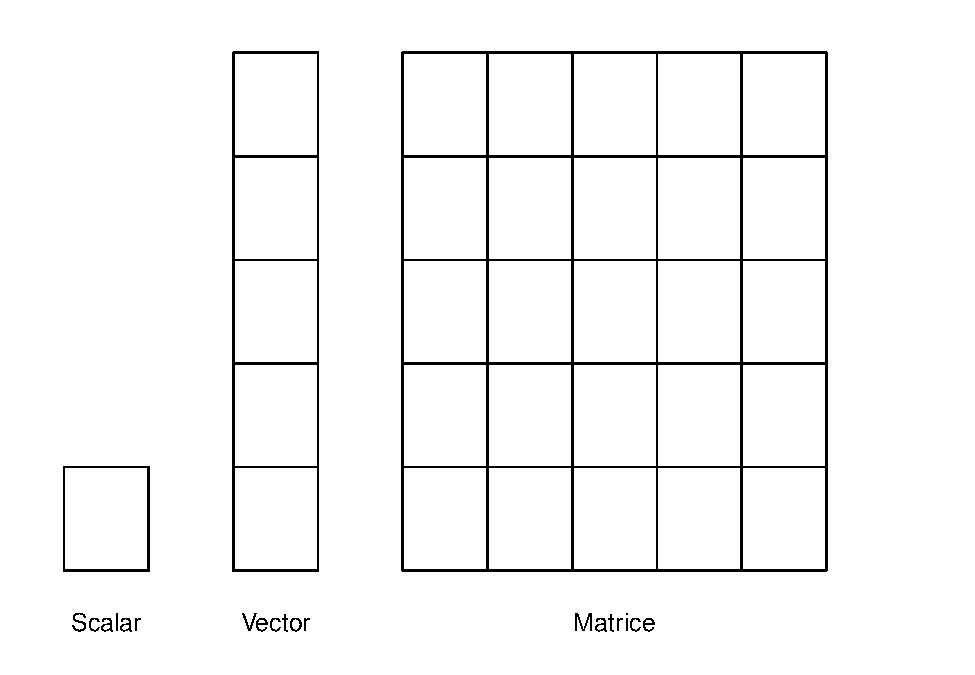
\includegraphics{Lab_1_pdf_files/figure-latex/unnamed-chunk-27-1} 

}

\caption{Scalari, Vectori, Matrice}\label{fig:unnamed-chunk-27}
\end{figure}

Indexarea liniilor și a coloanelor pentru o matrice începe cu 1. De
exemplu, elementul din colțul din stânga sus al unei matrice este notat
cu \texttt{x{[}1,1{]}}. De asemenea este important de menționat că
stocarea (internă) a metricelor se face pe coloane în sensul că prima
oară este stocată coloana 1, apoi coloana 2, etc..

Există mai multe moduri de creare a unei matrici în R. Funcțiile cele
mai uzuale sunt prezentate în tabelul de mai jos. Cum matricele sunt
combinații de vectori, fiecare funcție primește ca argument unul sau mai
mulți vectori (toți de același tip) și ne întoarce o matrice.

\begin{longtable}[]{@{}lll@{}}
\caption{Functii care permit crearea matricelor}\tabularnewline
\toprule
\begin{minipage}[b]{0.19\columnwidth}\raggedright\strut
Funcție\strut
\end{minipage} & \begin{minipage}[b]{0.27\columnwidth}\raggedright\strut
Descriere\strut
\end{minipage} & \begin{minipage}[b]{0.41\columnwidth}\raggedright\strut
Exemple\strut
\end{minipage}\tabularnewline
\midrule
\endfirsthead
\toprule
\begin{minipage}[b]{0.19\columnwidth}\raggedright\strut
Funcție\strut
\end{minipage} & \begin{minipage}[b]{0.27\columnwidth}\raggedright\strut
Descriere\strut
\end{minipage} & \begin{minipage}[b]{0.41\columnwidth}\raggedright\strut
Exemple\strut
\end{minipage}\tabularnewline
\midrule
\endhead
\begin{minipage}[t]{0.19\columnwidth}\raggedright\strut
\texttt{cbind(a,\ b,\ c)}\strut
\end{minipage} & \begin{minipage}[t]{0.27\columnwidth}\raggedright\strut
Combină vectorii ca și coloane într-o matrice\strut
\end{minipage} & \begin{minipage}[t]{0.41\columnwidth}\raggedright\strut
\texttt{cbind(1:5,\ 6:10,\ 11:15)}\strut
\end{minipage}\tabularnewline
\begin{minipage}[t]{0.19\columnwidth}\raggedright\strut
\texttt{rbind(a,\ b,\ c)}\strut
\end{minipage} & \begin{minipage}[t]{0.27\columnwidth}\raggedright\strut
Combină vectorii ca și linii într-o matrice\strut
\end{minipage} & \begin{minipage}[t]{0.41\columnwidth}\raggedright\strut
\texttt{rbind(1:5,\ 6:10,\ 11:15)}\strut
\end{minipage}\tabularnewline
\begin{minipage}[t]{0.19\columnwidth}\raggedright\strut
\texttt{matrix(x,\ nrow,\ ncol,\ byrow)}\strut
\end{minipage} & \begin{minipage}[t]{0.27\columnwidth}\raggedright\strut
Crează o matrice dintr-un vector \texttt{x}\strut
\end{minipage} & \begin{minipage}[t]{0.41\columnwidth}\raggedright\strut
\texttt{matrix(x\ =\ 1:12,\ nrow\ =\ 3,\ ncol\ =\ 4)}\strut
\end{minipage}\tabularnewline
\bottomrule
\end{longtable}

Pentru a vedea ce obținem atunci când folosim funcțiile \texttt{cbind()}
și \texttt{rbind()} să considerăm exemplele următoare:

\begin{Shaded}
\begin{Highlighting}[]
\NormalTok{x <-}\StringTok{ }\DecValTok{1}\OperatorTok{:}\DecValTok{5}
\NormalTok{y <-}\StringTok{ }\DecValTok{6}\OperatorTok{:}\DecValTok{10}
\NormalTok{z <-}\StringTok{ }\DecValTok{11}\OperatorTok{:}\DecValTok{15}

\CommentTok{# Cream o matrice cu x, y si z ca si coloane}
\KeywordTok{cbind}\NormalTok{(x, y, z)}
\end{Highlighting}
\end{Shaded}

\begin{verbatim}
##      x  y  z
## [1,] 1  6 11
## [2,] 2  7 12
## [3,] 3  8 13
## [4,] 4  9 14
## [5,] 5 10 15
\end{verbatim}

\begin{Shaded}
\begin{Highlighting}[]
\CommentTok{# Cream o matrice in care x, y si z sunt linii}
\KeywordTok{rbind}\NormalTok{(x, y, z)}
\end{Highlighting}
\end{Shaded}

\begin{verbatim}
##   [,1] [,2] [,3] [,4] [,5]
## x    1    2    3    4    5
## y    6    7    8    9   10
## z   11   12   13   14   15
\end{verbatim}

Funcția \texttt{matrix()} crează o matrice plecând de la un singur
vector. Funcția are patru valori de intrare: \texttt{data} -- un vector
cu date, \texttt{nrow} -- numărul de linii pe care le vrem în matrice,
\texttt{ncol} -- numărul de coloane pe care să le aibe matricea și
\texttt{byrow} -- o valoare logică care permite crearea matricei pe
linii (nu pe coloane cum este default-ul).

\begin{Shaded}
\begin{Highlighting}[]
\CommentTok{# matrice cu 5 linii si 2 coloane}
\KeywordTok{matrix}\NormalTok{(}\DataTypeTok{data =} \DecValTok{1}\OperatorTok{:}\DecValTok{10}\NormalTok{,}
       \DataTypeTok{nrow =} \DecValTok{5}\NormalTok{,}
       \DataTypeTok{ncol =} \DecValTok{2}\NormalTok{)}
\end{Highlighting}
\end{Shaded}

\begin{verbatim}
##      [,1] [,2]
## [1,]    1    6
## [2,]    2    7
## [3,]    3    8
## [4,]    4    9
## [5,]    5   10
\end{verbatim}

\begin{Shaded}
\begin{Highlighting}[]
\CommentTok{# matrice cu 2 linii si 5 coloane}
\KeywordTok{matrix}\NormalTok{(}\DataTypeTok{data =} \DecValTok{1}\OperatorTok{:}\DecValTok{10}\NormalTok{,}
       \DataTypeTok{nrow =} \DecValTok{2}\NormalTok{,}
       \DataTypeTok{ncol =} \DecValTok{5}\NormalTok{)}
\end{Highlighting}
\end{Shaded}

\begin{verbatim}
##      [,1] [,2] [,3] [,4] [,5]
## [1,]    1    3    5    7    9
## [2,]    2    4    6    8   10
\end{verbatim}

\begin{Shaded}
\begin{Highlighting}[]
\CommentTok{# aceeasi matrice cu 2 linii si 5 coloane, umpluta pe linii }
\KeywordTok{matrix}\NormalTok{(}\DataTypeTok{data =} \DecValTok{1}\OperatorTok{:}\DecValTok{10}\NormalTok{,}
       \DataTypeTok{nrow =} \DecValTok{2}\NormalTok{,}
       \DataTypeTok{ncol =} \DecValTok{5}\NormalTok{,}
       \DataTypeTok{byrow =} \OtherTok{TRUE}\NormalTok{)}
\end{Highlighting}
\end{Shaded}

\begin{verbatim}
##      [,1] [,2] [,3] [,4] [,5]
## [1,]    1    2    3    4    5
## [2,]    6    7    8    9   10
\end{verbatim}

Operațiile uzuale cu vectori se aplică și matricelor. Pe lângă acestea
avem la dispoziție și operații de algebră liniară clasice, cum ar fi
determinarea dimensiunii acestora, transpunerea matricelor sau
înmulțirea lor:

\begin{Shaded}
\begin{Highlighting}[]
\NormalTok{m =}\StringTok{ }\KeywordTok{matrix}\NormalTok{(}\DataTypeTok{data =} \DecValTok{1}\OperatorTok{:}\DecValTok{10}\NormalTok{,}
       \DataTypeTok{nrow =} \DecValTok{2}\NormalTok{,}
       \DataTypeTok{ncol =} \DecValTok{5}\NormalTok{)}
\NormalTok{m}
\end{Highlighting}
\end{Shaded}

\begin{verbatim}
##      [,1] [,2] [,3] [,4] [,5]
## [1,]    1    3    5    7    9
## [2,]    2    4    6    8   10
\end{verbatim}

\begin{Shaded}
\begin{Highlighting}[]
\KeywordTok{dim}\NormalTok{(m) }\CommentTok{# dimensiunea matricei}
\end{Highlighting}
\end{Shaded}

\begin{verbatim}
## [1] 2 5
\end{verbatim}

\begin{Shaded}
\begin{Highlighting}[]
\KeywordTok{nrow}\NormalTok{(m) }\CommentTok{# numarul de linii}
\end{Highlighting}
\end{Shaded}

\begin{verbatim}
## [1] 2
\end{verbatim}

\begin{Shaded}
\begin{Highlighting}[]
\KeywordTok{ncol}\NormalTok{(m) }\CommentTok{# numarul de coloane}
\end{Highlighting}
\end{Shaded}

\begin{verbatim}
## [1] 5
\end{verbatim}

\begin{Shaded}
\begin{Highlighting}[]
\NormalTok{tpm =}\StringTok{ }\KeywordTok{t}\NormalTok{(m) }\CommentTok{# transpusa}
\NormalTok{tpm}
\end{Highlighting}
\end{Shaded}

\begin{verbatim}
##      [,1] [,2]
## [1,]    1    2
## [2,]    3    4
## [3,]    5    6
## [4,]    7    8
## [5,]    9   10
\end{verbatim}

\begin{Shaded}
\begin{Highlighting}[]
\NormalTok{m }\OperatorTok\StringTok{ }\NormalTok{tpm }\CommentTok{# inmultirea matricelor}
\end{Highlighting}
\end{Shaded}

\begin{verbatim}
##      [,1] [,2]
## [1,]  165  190
## [2,]  190  220
\end{verbatim}

Metodele de indexare discutate pentru vectori se aplică și în cazul
matricelor (\texttt{{[},{]}}) numai că acum în loc să folosim un vector
să indexăm putem să folosim doi vectori. Sintaxa are structura generală
\texttt{m{[}linii,\ coloane{]}} unde \texttt{linii} și \texttt{coloane}
sunt vectori cu valori întregi.

\begin{Shaded}
\begin{Highlighting}[]
\NormalTok{m =}\StringTok{ }\KeywordTok{matrix}\NormalTok{(}\DecValTok{1}\OperatorTok{:}\DecValTok{20}\NormalTok{, }\DataTypeTok{nrow =} \DecValTok{4}\NormalTok{, }\DataTypeTok{byrow =} \OtherTok{TRUE}\NormalTok{)}

\CommentTok{# Linia 1}
\NormalTok{m[}\DecValTok{1}\NormalTok{, ]}
\end{Highlighting}
\end{Shaded}

\begin{verbatim}
## [1] 1 2 3 4 5
\end{verbatim}

\begin{Shaded}
\begin{Highlighting}[]
\CommentTok{# Coloana 5}
\NormalTok{m[, }\DecValTok{5}\NormalTok{]}
\end{Highlighting}
\end{Shaded}

\begin{verbatim}
## [1]  5 10 15 20
\end{verbatim}

\begin{Shaded}
\begin{Highlighting}[]
\CommentTok{# Liniile 2, 3 si coloanele 3, 4}
\NormalTok{m[}\DecValTok{2}\OperatorTok{:}\DecValTok{3}\NormalTok{, }\DecValTok{3}\OperatorTok{:}\DecValTok{4}\NormalTok{]}
\end{Highlighting}
\end{Shaded}

\begin{verbatim}
##      [,1] [,2]
## [1,]    8    9
## [2,]   13   14
\end{verbatim}

\begin{Shaded}
\begin{Highlighting}[]
\CommentTok{# Elementele din coloana 3 care corespund liniilor pentru care elementele de pe prima coloana sunt > 3}
\NormalTok{m[m[,}\DecValTok{1}\NormalTok{]}\OperatorTok{>}\DecValTok{3}\NormalTok{, }\DecValTok{3}\NormalTok{]}
\end{Highlighting}
\end{Shaded}

\begin{verbatim}
## [1]  8 13 18
\end{verbatim}

\subsection{Liste}\label{liste}

Spre deosebire de vectori în care toate elementele trebuie să aibă
același tip de dată, structura de dată din R de tip listă (\emph{list})
permite combinarea obiectelor de mai multe tipuri. Cu alte cuvinte, o
listă poate avea primul element un scalar, al doilea un vector, al
treilea o matrice iar cel de-al patrulea element poate fi o altă listă.
Tehnic listele sunt tot vectori, vectorii pe care i-am văzut anterior se
numesc \emph{vectori atomici}, deoarece elementele lor nu se pot diviza,
pe când listele se numesc \emph{vectori recursivi}.

Ca un prim exemplu să considerăm cazul unei baze de date de angajați.
Pentru fiecare angajat, ne dorim să stocăm numele angajatului (șir de
caractere), salariul (valoare numerică) și o valoare de tip logic care
poate reprezenta apartenența într-o asociație. Pentru crearea listei
folosim funcția \texttt{list()}:

\begin{Shaded}
\begin{Highlighting}[]
\NormalTok{a =}\StringTok{ }\KeywordTok{list}\NormalTok{(}\DataTypeTok{nume =} \StringTok{"Ionel"}\NormalTok{, }\DataTypeTok{salariu =} \DecValTok{1500}\NormalTok{, }\DataTypeTok{apartenenta =}\NormalTok{ T)}
\NormalTok{a}
\end{Highlighting}
\end{Shaded}

\begin{verbatim}
## $nume
## [1] "Ionel"
## 
## $salariu
## [1] 1500
## 
## $apartenenta
## [1] TRUE
\end{verbatim}

\begin{Shaded}
\begin{Highlighting}[]
\KeywordTok{str}\NormalTok{(a) }\CommentTok{# structura listei}
\end{Highlighting}
\end{Shaded}

\begin{verbatim}
## List of 3
##  $ nume       : chr "Ionel"
##  $ salariu    : num 1500
##  $ apartenenta: logi TRUE
\end{verbatim}

\begin{Shaded}
\begin{Highlighting}[]
\KeywordTok{names}\NormalTok{(a) }\CommentTok{# numele listei}
\end{Highlighting}
\end{Shaded}

\begin{verbatim}
## [1] "nume"        "salariu"     "apartenenta"
\end{verbatim}

Numele componentelor listei \texttt{a} (nume, salariu, apartenenta) nu
sunt obligatorii dar cu toate acestea pentru claritate sunt indicate:

\begin{Shaded}
\begin{Highlighting}[]
\NormalTok{a2 =}\StringTok{ }\KeywordTok{list}\NormalTok{(}\StringTok{"Ionel"}\NormalTok{, }\DecValTok{1500}\NormalTok{, T)}
\NormalTok{a2}
\end{Highlighting}
\end{Shaded}

\begin{verbatim}
## [[1]]
## [1] "Ionel"
## 
## [[2]]
## [1] 1500
## 
## [[3]]
## [1] TRUE
\end{verbatim}

Deoarece listele sunt vectori ele pot fi create și prin intermediul
funcției \texttt{vector()}:

\begin{Shaded}
\begin{Highlighting}[]
\NormalTok{z <-}\StringTok{ }\KeywordTok{vector}\NormalTok{(}\DataTypeTok{mode=}\StringTok{"list"}\NormalTok{)}
\NormalTok{z}
\end{Highlighting}
\end{Shaded}

\begin{verbatim}
## list()
\end{verbatim}

\begin{Shaded}
\begin{Highlighting}[]
\NormalTok{z[[}\StringTok{"a"}\NormalTok{]] =}\StringTok{ }\DecValTok{3}
\NormalTok{z}
\end{Highlighting}
\end{Shaded}

\begin{verbatim}
## $a
## [1] 3
\end{verbatim}

\subsubsection{Indexarea listelor}\label{indexarea-listelor}

Elementele unei liste pot fi accesate în diferite moduri. Dacă dorim să
extragem primul element al listei atunci vom folosi indexarea care
folosește o singură pereche de paranteze pătrate \texttt{{[}{]}}

\begin{Shaded}
\begin{Highlighting}[]
\NormalTok{a[}\DecValTok{1}\NormalTok{]}
\end{Highlighting}
\end{Shaded}

\begin{verbatim}
## $nume
## [1] "Ionel"
\end{verbatim}

\begin{Shaded}
\begin{Highlighting}[]
\NormalTok{a[}\DecValTok{2}\NormalTok{]}
\end{Highlighting}
\end{Shaded}

\begin{verbatim}
## $salariu
## [1] 1500
\end{verbatim}

\begin{Shaded}
\begin{Highlighting}[]
\CommentTok{# ce obtinem cand extragem un element al listei a ?}
\KeywordTok{str}\NormalTok{(a[}\DecValTok{1}\NormalTok{]) }
\end{Highlighting}
\end{Shaded}

\begin{verbatim}
## List of 1
##  $ nume: chr "Ionel"
\end{verbatim}

În cazul în care vrem să accesăm structura de date corespunzătoare
elementului i al listei vom folosi două perechi de paranteze pătrate
\texttt{{[}{[}{]}{]}} sau în cazul în care lista are nume operatorul
\texttt{\$} urmat de numele elementului i.

\begin{Shaded}
\begin{Highlighting}[]
\NormalTok{a[[}\DecValTok{1}\NormalTok{]]}
\end{Highlighting}
\end{Shaded}

\begin{verbatim}
## [1] "Ionel"
\end{verbatim}

\begin{Shaded}
\begin{Highlighting}[]
\NormalTok{a[[}\DecValTok{2}\NormalTok{]]}
\end{Highlighting}
\end{Shaded}

\begin{verbatim}
## [1] 1500
\end{verbatim}

\begin{Shaded}
\begin{Highlighting}[]
\NormalTok{a}\OperatorTok{$}\NormalTok{nume}
\end{Highlighting}
\end{Shaded}

\begin{verbatim}
## [1] "Ionel"
\end{verbatim}

\begin{Shaded}
\begin{Highlighting}[]
\NormalTok{a[[}\StringTok{"nume"}\NormalTok{]]}
\end{Highlighting}
\end{Shaded}

\begin{verbatim}
## [1] "Ionel"
\end{verbatim}

Operațiile de adăugare, respectiv ștergere, a elementelor unei liste
sunt des întâlnite.

Putem adăuga elemente după ce o listă a fost creată folosind numele
componentei

\begin{Shaded}
\begin{Highlighting}[]
\NormalTok{z =}\StringTok{ }\KeywordTok{list}\NormalTok{(}\DataTypeTok{a =} \StringTok{"abc"}\NormalTok{, }\DataTypeTok{b =} \DecValTok{111}\NormalTok{, }\DataTypeTok{c =} \KeywordTok{c}\NormalTok{(}\OtherTok{TRUE}\NormalTok{, }\OtherTok{FALSE}\NormalTok{))}
\NormalTok{z}
\end{Highlighting}
\end{Shaded}

\begin{verbatim}
## $a
## [1] "abc"
## 
## $b
## [1] 111
## 
## $c
## [1]  TRUE FALSE
\end{verbatim}

\begin{Shaded}
\begin{Highlighting}[]
\NormalTok{z}\OperatorTok{$}\NormalTok{d =}\StringTok{ "un nou element"}
\NormalTok{z}
\end{Highlighting}
\end{Shaded}

\begin{verbatim}
## $a
## [1] "abc"
## 
## $b
## [1] 111
## 
## $c
## [1]  TRUE FALSE
## 
## $d
## [1] "un nou element"
\end{verbatim}

sau indexare vectorială

\begin{Shaded}
\begin{Highlighting}[]
\NormalTok{z[[}\DecValTok{5}\NormalTok{]] =}\StringTok{ }\DecValTok{200}
\NormalTok{z[}\DecValTok{6}\OperatorTok{:}\DecValTok{7}\NormalTok{] =}\StringTok{ }\KeywordTok{c}\NormalTok{(}\StringTok{"unu"}\NormalTok{, }\StringTok{"doi"}\NormalTok{)}
\NormalTok{z}
\end{Highlighting}
\end{Shaded}

\begin{verbatim}
## $a
## [1] "abc"
## 
## $b
## [1] 111
## 
## $c
## [1]  TRUE FALSE
## 
## $d
## [1] "un nou element"
## 
## [[5]]
## [1] 200
## 
## [[6]]
## [1] "unu"
## 
## [[7]]
## [1] "doi"
\end{verbatim}

Putem șterge o componentă a listei atribuindu-i valoarea \texttt{NULL}:

\begin{Shaded}
\begin{Highlighting}[]
\NormalTok{z[}\DecValTok{4}\NormalTok{] =}\StringTok{ }\OtherTok{NULL}
\NormalTok{z}
\end{Highlighting}
\end{Shaded}

\begin{verbatim}
## $a
## [1] "abc"
## 
## $b
## [1] 111
## 
## $c
## [1]  TRUE FALSE
## 
## [[4]]
## [1] 200
## 
## [[5]]
## [1] "unu"
## 
## [[6]]
## [1] "doi"
\end{verbatim}

Putem de asemenea să concatenăm două liste folosind funcția \texttt{c()}
și să determinăm lungimea noii liste cu funcția \texttt{length()}.

\begin{Shaded}
\begin{Highlighting}[]
\NormalTok{l1 =}\StringTok{ }\KeywordTok{list}\NormalTok{(}\DecValTok{1}\OperatorTok{:}\DecValTok{10}\NormalTok{, }\KeywordTok{matrix}\NormalTok{(}\DecValTok{1}\OperatorTok{:}\DecValTok{6}\NormalTok{, }\DataTypeTok{ncol =} \DecValTok{3}\NormalTok{), }\KeywordTok{c}\NormalTok{(T, F))}
\NormalTok{l2 =}\StringTok{ }\KeywordTok{list}\NormalTok{(}\KeywordTok{c}\NormalTok{(}\StringTok{"Ionel"}\NormalTok{, }\StringTok{"Maria"}\NormalTok{), }\KeywordTok{seq}\NormalTok{(}\DecValTok{1}\NormalTok{,}\DecValTok{10}\NormalTok{,}\DecValTok{2}\NormalTok{))}

\NormalTok{l3 =}\StringTok{ }\KeywordTok{c}\NormalTok{(l1, l2)}
\KeywordTok{length}\NormalTok{(l3)}
\end{Highlighting}
\end{Shaded}

\begin{verbatim}
## [1] 5
\end{verbatim}

\begin{Shaded}
\begin{Highlighting}[]
\KeywordTok{str}\NormalTok{(l3)}
\end{Highlighting}
\end{Shaded}

\begin{verbatim}
## List of 5
##  $ : int [1:10] 1 2 3 4 5 6 7 8 9 10
##  $ : int [1:2, 1:3] 1 2 3 4 5 6
##  $ : logi [1:2] TRUE FALSE
##  $ : chr [1:2] "Ionel" "Maria"
##  $ : num [1:5] 1 3 5 7 9
\end{verbatim}

\subsection{Data frame-uri}\label{data-frame-uri}

La nivel intuitiv, o structură de date de tip \emph{data frame} este ca
o matrice, având o structură bidimensională cu linii și coloane. Cu
toate acestea ea diferă de structura de date de tip matrice prin faptul
că fiecare coloană poate avea tipuri de date diferite. Spre exemplu, o
coloană poate să conțină valori numerice pe când o alta, valori de tip
caracter sau logic. Din punct de vedere tehnic, o structură de tip data
frame este o listă a cărei componente sunt vectori (atomici) de lungimi
egale.

Pentru a crea un dataframe din vectori putem folosi funcția
\texttt{data.frame()}. Această funcție funcționează similar cu funcția
\texttt{list()} sau \texttt{cbind()}, diferența față de \texttt{cbind()}
este că avem posibilitatea să dăm nume coloanelor atunci când le unim.
Dată fiind flexibilitatea acestei structuri de date, majoritatea
seturilor de date din R sunt stocate sub formă de dataframe (această
structură de date este și cea mai des întâlnită în analiza statistică).

Să creăm un dataframe simplu numit \texttt{survey} folosind funcția
\texttt{data.frame()}:

\begin{Shaded}
\begin{Highlighting}[]
\NormalTok{survey <-}\StringTok{ }\KeywordTok{data.frame}\NormalTok{(}\StringTok{"index"}\NormalTok{ =}\StringTok{ }\KeywordTok{c}\NormalTok{(}\DecValTok{1}\NormalTok{, }\DecValTok{2}\NormalTok{, }\DecValTok{3}\NormalTok{, }\DecValTok{4}\NormalTok{, }\DecValTok{5}\NormalTok{),}
                     \StringTok{"sex"}\NormalTok{ =}\StringTok{ }\KeywordTok{c}\NormalTok{(}\StringTok{"m"}\NormalTok{, }\StringTok{"m"}\NormalTok{, }\StringTok{"m"}\NormalTok{, }\StringTok{"f"}\NormalTok{, }\StringTok{"f"}\NormalTok{),}
                     \StringTok{"age"}\NormalTok{ =}\StringTok{ }\KeywordTok{c}\NormalTok{(}\DecValTok{99}\NormalTok{, }\DecValTok{46}\NormalTok{, }\DecValTok{23}\NormalTok{, }\DecValTok{54}\NormalTok{, }\DecValTok{23}\NormalTok{))}
\NormalTok{survey}
\end{Highlighting}
\end{Shaded}

\begin{verbatim}
##   index sex age
## 1     1   m  99
## 2     2   m  46
## 3     3   m  23
## 4     4   f  54
## 5     5   f  23
\end{verbatim}

Funcția \texttt{data.frame()} prezintă un argument specific numit
\texttt{stringsAsFactors} care permite convertirea coloanelor ce conțin
elemente de tip caracter într-un tip de obiect numit \textbf{factor}. Un
factor este o variabilă nominală care poate lua un număr bine definit de
valori. De exemplu, putem crea o variabilă de tip factor \emph{sex} care
poate lua doar două valori: \emph{masculin} și \emph{feminin}.
Comportamentul implicit al funcției \texttt{data.frame()}
(\texttt{stringAsFactors\ =\ TRUE}) transformă automat coloanele de tip
caracter în factor, motiv pentru care trebuie să includem argumentul
\texttt{stringsAsFactors\ =\ FALSE}.

\begin{Shaded}
\begin{Highlighting}[]
\CommentTok{# Structura initiala}
\KeywordTok{str}\NormalTok{(survey)}
\end{Highlighting}
\end{Shaded}

\begin{verbatim}
## 'data.frame':    5 obs. of  3 variables:
##  $ index: num  1 2 3 4 5
##  $ sex  : Factor w/ 2 levels "f","m": 2 2 2 1 1
##  $ age  : num  99 46 23 54 23
\end{verbatim}

\begin{Shaded}
\begin{Highlighting}[]
\NormalTok{survey <-}\StringTok{ }\KeywordTok{data.frame}\NormalTok{(}\StringTok{"index"}\NormalTok{ =}\StringTok{ }\KeywordTok{c}\NormalTok{(}\DecValTok{1}\NormalTok{, }\DecValTok{2}\NormalTok{, }\DecValTok{3}\NormalTok{, }\DecValTok{4}\NormalTok{, }\DecValTok{5}\NormalTok{),}
                     \StringTok{"sex"}\NormalTok{ =}\StringTok{ }\KeywordTok{c}\NormalTok{(}\StringTok{"m"}\NormalTok{, }\StringTok{"m"}\NormalTok{, }\StringTok{"m"}\NormalTok{, }\StringTok{"f"}\NormalTok{, }\StringTok{"f"}\NormalTok{),}
                     \StringTok{"age"}\NormalTok{ =}\StringTok{ }\KeywordTok{c}\NormalTok{(}\DecValTok{99}\NormalTok{, }\DecValTok{46}\NormalTok{, }\DecValTok{23}\NormalTok{, }\DecValTok{54}\NormalTok{, }\DecValTok{23}\NormalTok{),}
                     \DataTypeTok{stringsAsFactors =} \OtherTok{FALSE}\NormalTok{)}

\CommentTok{# Structura de dupa }
\KeywordTok{str}\NormalTok{(survey)}
\end{Highlighting}
\end{Shaded}

\begin{verbatim}
## 'data.frame':    5 obs. of  3 variables:
##  $ index: num  1 2 3 4 5
##  $ sex  : chr  "m" "m" "m" "f" ...
##  $ age  : num  99 46 23 54 23
\end{verbatim}

R are mai multe funcții care permit vizualizarea structurilor de tip
dataframe. Table de mai jos include câteva astfel de funcții:

\begin{longtable}[]{@{}ll@{}}
\caption{Exemple de functii necesare pentru intelegerea structurii
dataframe-ului}\tabularnewline
\toprule
Funcție & Descriere\tabularnewline
\midrule
\endfirsthead
\toprule
Funcție & Descriere\tabularnewline
\midrule
\endhead
\texttt{head(x),\ tail(x)} & Printarea primelor linii (sau ultimelor
linii).\tabularnewline
\texttt{View(x)} & Vizualizarea obiectului într-o fereastră nouă,
tabelară.\tabularnewline
\texttt{nrow(x),\ ncol(x),\ dim(x)} & Numărul de linii și de
coloane.\tabularnewline
\texttt{rownames(),\ colnames(),\ names()} & Numele liniilor sau
coloanelor.\tabularnewline
\texttt{str(x)} & Structura dataframe-ului\tabularnewline
\bottomrule
\end{longtable}

\begin{Shaded}
\begin{Highlighting}[]
\KeywordTok{data}\NormalTok{() }\CommentTok{# vedem ce seturi de date exista}

\CommentTok{# Alegem setul de date mtcars}
\NormalTok{?mtcars}
\end{Highlighting}
\end{Shaded}

\begin{verbatim}
## starting httpd help server ... done
\end{verbatim}

\begin{Shaded}
\begin{Highlighting}[]
\KeywordTok{str}\NormalTok{(mtcars) }\CommentTok{# structura setului de date}
\end{Highlighting}
\end{Shaded}

\begin{verbatim}
## 'data.frame':    32 obs. of  11 variables:
##  $ mpg : num  21 21 22.8 21.4 18.7 18.1 14.3 24.4 22.8 19.2 ...
##  $ cyl : num  6 6 4 6 8 6 8 4 4 6 ...
##  $ disp: num  160 160 108 258 360 ...
##  $ hp  : num  110 110 93 110 175 105 245 62 95 123 ...
##  $ drat: num  3.9 3.9 3.85 3.08 3.15 2.76 3.21 3.69 3.92 3.92 ...
##  $ wt  : num  2.62 2.88 2.32 3.21 3.44 ...
##  $ qsec: num  16.5 17 18.6 19.4 17 ...
##  $ vs  : num  0 0 1 1 0 1 0 1 1 1 ...
##  $ am  : num  1 1 1 0 0 0 0 0 0 0 ...
##  $ gear: num  4 4 4 3 3 3 3 4 4 4 ...
##  $ carb: num  4 4 1 1 2 1 4 2 2 4 ...
\end{verbatim}

\begin{Shaded}
\begin{Highlighting}[]
\KeywordTok{head}\NormalTok{(mtcars)}
\end{Highlighting}
\end{Shaded}

\begin{verbatim}
##                    mpg cyl disp  hp drat    wt  qsec vs am gear carb
## Mazda RX4         21.0   6  160 110 3.90 2.620 16.46  0  1    4    4
## Mazda RX4 Wag     21.0   6  160 110 3.90 2.875 17.02  0  1    4    4
## Datsun 710        22.8   4  108  93 3.85 2.320 18.61  1  1    4    1
## Hornet 4 Drive    21.4   6  258 110 3.08 3.215 19.44  1  0    3    1
## Hornet Sportabout 18.7   8  360 175 3.15 3.440 17.02  0  0    3    2
## Valiant           18.1   6  225 105 2.76 3.460 20.22  1  0    3    1
\end{verbatim}

\begin{Shaded}
\begin{Highlighting}[]
\KeywordTok{tail}\NormalTok{(mtcars)}
\end{Highlighting}
\end{Shaded}

\begin{verbatim}
##                 mpg cyl  disp  hp drat    wt qsec vs am gear carb
## Porsche 914-2  26.0   4 120.3  91 4.43 2.140 16.7  0  1    5    2
## Lotus Europa   30.4   4  95.1 113 3.77 1.513 16.9  1  1    5    2
## Ford Pantera L 15.8   8 351.0 264 4.22 3.170 14.5  0  1    5    4
## Ferrari Dino   19.7   6 145.0 175 3.62 2.770 15.5  0  1    5    6
## Maserati Bora  15.0   8 301.0 335 3.54 3.570 14.6  0  1    5    8
## Volvo 142E     21.4   4 121.0 109 4.11 2.780 18.6  1  1    4    2
\end{verbatim}

\begin{Shaded}
\begin{Highlighting}[]
\KeywordTok{rownames}\NormalTok{(mtcars)}
\end{Highlighting}
\end{Shaded}

\begin{verbatim}
##  [1] "Mazda RX4"           "Mazda RX4 Wag"       "Datsun 710"         
##  [4] "Hornet 4 Drive"      "Hornet Sportabout"   "Valiant"            
##  [7] "Duster 360"          "Merc 240D"           "Merc 230"           
## [10] "Merc 280"            "Merc 280C"           "Merc 450SE"         
## [13] "Merc 450SL"          "Merc 450SLC"         "Cadillac Fleetwood" 
## [16] "Lincoln Continental" "Chrysler Imperial"   "Fiat 128"           
## [19] "Honda Civic"         "Toyota Corolla"      "Toyota Corona"      
## [22] "Dodge Challenger"    "AMC Javelin"         "Camaro Z28"         
## [25] "Pontiac Firebird"    "Fiat X1-9"           "Porsche 914-2"      
## [28] "Lotus Europa"        "Ford Pantera L"      "Ferrari Dino"       
## [31] "Maserati Bora"       "Volvo 142E"
\end{verbatim}

\begin{Shaded}
\begin{Highlighting}[]
\KeywordTok{names}\NormalTok{(mtcars)}
\end{Highlighting}
\end{Shaded}

\begin{verbatim}
##  [1] "mpg"  "cyl"  "disp" "hp"   "drat" "wt"   "qsec" "vs"   "am"   "gear"
## [11] "carb"
\end{verbatim}

\begin{Shaded}
\begin{Highlighting}[]
\KeywordTok{View}\NormalTok{(mtcars) }
\end{Highlighting}
\end{Shaded}

\subsubsection{Metode de indexare}\label{metode-de-indexare}

Indexarea structurilor de tip dataframe se face la fel ca și indexarea
listelor.

\begin{Shaded}
\begin{Highlighting}[]
\NormalTok{mtcars[}\DecValTok{1}\NormalTok{,}\DecValTok{1}\OperatorTok{:}\DecValTok{4}\NormalTok{]}
\end{Highlighting}
\end{Shaded}

\begin{verbatim}
##           mpg cyl disp  hp
## Mazda RX4  21   6  160 110
\end{verbatim}

\begin{Shaded}
\begin{Highlighting}[]
\NormalTok{mtcars[}\KeywordTok{c}\NormalTok{(}\DecValTok{1}\NormalTok{,}\DecValTok{2}\NormalTok{),}\DecValTok{2}\NormalTok{]}
\end{Highlighting}
\end{Shaded}

\begin{verbatim}
## [1] 6 6
\end{verbatim}

\begin{Shaded}
\begin{Highlighting}[]
\NormalTok{mtcars}\OperatorTok{$}\NormalTok{mpg}
\end{Highlighting}
\end{Shaded}

\begin{verbatim}
##  [1] 21.0 21.0 22.8 21.4 18.7 18.1 14.3 24.4 22.8 19.2 17.8 16.4 17.3 15.2
## [15] 10.4 10.4 14.7 32.4 30.4 33.9 21.5 15.5 15.2 13.3 19.2 27.3 26.0 30.4
## [29] 15.8 19.7 15.0 21.4
\end{verbatim}

La fel ca vectorii, dataframe-urile (dar și listele) pot fi indexate
logic

\begin{Shaded}
\begin{Highlighting}[]
\NormalTok{mtcars[mtcars}\OperatorTok{$}\NormalTok{mpg }\OperatorTok{>}\StringTok{ }\DecValTok{25}\NormalTok{, ]}
\end{Highlighting}
\end{Shaded}

\begin{verbatim}
##                 mpg cyl  disp  hp drat    wt  qsec vs am gear carb
## Fiat 128       32.4   4  78.7  66 4.08 2.200 19.47  1  1    4    1
## Honda Civic    30.4   4  75.7  52 4.93 1.615 18.52  1  1    4    2
## Toyota Corolla 33.9   4  71.1  65 4.22 1.835 19.90  1  1    4    1
## Fiat X1-9      27.3   4  79.0  66 4.08 1.935 18.90  1  1    4    1
## Porsche 914-2  26.0   4 120.3  91 4.43 2.140 16.70  0  1    5    2
## Lotus Europa   30.4   4  95.1 113 3.77 1.513 16.90  1  1    5    2
\end{verbatim}

\begin{Shaded}
\begin{Highlighting}[]
\NormalTok{mtcars[(mtcars}\OperatorTok{$}\NormalTok{mpg }\OperatorTok{>}\StringTok{ }\DecValTok{25}\NormalTok{) }\OperatorTok{&}\StringTok{ }\NormalTok{(mtcars}\OperatorTok{$}\NormalTok{wt }\OperatorTok{<}\StringTok{ }\FloatTok{1.8}\NormalTok{), ]}
\end{Highlighting}
\end{Shaded}

\begin{verbatim}
##               mpg cyl disp  hp drat    wt  qsec vs am gear carb
## Honda Civic  30.4   4 75.7  52 4.93 1.615 18.52  1  1    4    2
## Lotus Europa 30.4   4 95.1 113 3.77 1.513 16.90  1  1    5    2
\end{verbatim}

O altă metodă de indexare este prin folosirea funcției
\texttt{subset()}.

\begin{longtable}[]{@{}ll@{}}
\caption{Principalele argumente ale functiei subset()}\tabularnewline
\toprule
Argument & Descriere\tabularnewline
\midrule
\endfirsthead
\toprule
Argument & Descriere\tabularnewline
\midrule
\endhead
\texttt{x} & Un dataframe\tabularnewline
\texttt{subset} & Un vector logic care indică liniile pe care le
vrem\tabularnewline
\texttt{select} & Coloanele pe care vrem să le păstrăm\tabularnewline
\bottomrule
\end{longtable}

\begin{Shaded}
\begin{Highlighting}[]
\KeywordTok{subset}\NormalTok{(}\DataTypeTok{x =}\NormalTok{ mtcars,}
      \DataTypeTok{subset =}\NormalTok{ mpg }\OperatorTok{<}\StringTok{ }\DecValTok{12} \OperatorTok{&}
\StringTok{               }\NormalTok{cyl }\OperatorTok{>}\StringTok{ }\DecValTok{6}\NormalTok{,}
      \DataTypeTok{select =} \KeywordTok{c}\NormalTok{(disp, wt))}
\end{Highlighting}
\end{Shaded}

\begin{verbatim}
##                     disp    wt
## Cadillac Fleetwood   472 5.250
## Lincoln Continental  460 5.424
\end{verbatim}


\end{document}
